\documentclass{article}
\usepackage{graphicx}
\usepackage{float}
\usepackage{subfigure}
\usepackage{subcaption}
\usepackage{fancyhdr} 
\usepackage{caption}
\usepackage{hyperref}
\usepackage{amssymb}
\usepackage{amsmath}
\pagestyle{fancy}
\fancyhead[RO]{Emanuele Zanusso }
\fancyhead[LO]{TANS 2025}

\title{TANS 2025 - Zanusso}
\author{Emanuele Zanusso}
\date{2024-2025}
\renewcommand*\contentsname{Indice}

\begin{document}
\maketitle
\tableofcontents
\newpage

\section{Introduzione e macrostruttura}
Il presente progetto inscena i processi di simulazione e ricostruzione FAST2, che avvengono in un esperimento a collider, nell'ipotesi che le particelle siano ultra relativistiche. Quest'ultima permette di trascurare l'effetto di un ipotetico campo magnetico, implicando solo traiettorie rettilinee. 
$\\$
Esso si articola in 4 directories principali:
\begin{itemize}

\item \textbf{work\textunderscore TANS}:  custodisce il cuore della consegna, ossia le macro per avviare la simulazione, la rivelazione, la ricostruzione e per realizzare un event display degli eventi simulati
\item \textbf{classes\textunderscore TANS}:  vi sono le classi impiegate durante lo svolgimento della consegna
\item \textbf{dat\textunderscore TANS}: raccoglie le distribuzioni utili sulla cinematica delle particelle, oltre ai risultati (organizzati in TTree) delle suddette fasi, conservati all'interno di file .root
\item \textbf{results\textunderscore TANS}: raccoglie le macro per la produzione dei risultati relativi alle performance

\end{itemize}

\section{Classi}

\subsection{points\textunderscore TANS}
\begin{itemize}
\item \textbf{cPoint}: implementa il concetto di punto (x, y, z) in coordinate cartesiane
\item \textbf{cilPoint}: classe che implementa il concetto di punto (R, $\phi$, Z) in coordinate cilindriche. Utile per lo sparpagliamento dovuto allo smearing
\item \textbf{pAng}: classe di supporto per trattare gli angoli, soprattutto  per collegare la grandezza pseudorapidità $\eta$ all'angolo $\theta$

\end{itemize}

\subsection{detectors\textunderscore TANS}
\begin{itemize}
\item \textbf{dLayer}: classe che implementa il concetto di detector di raggio r, lunghezza l e spessore w. Costruisce anche l'ambiente per l'event display, sfruttando la classe TGeo
\item \textbf{smLayer}: classe di supporto che implementa lo smearing dovuto al processo di rivelazione e di generazione di rumore nei rivelatori

\end{itemize}

\subsection{phy\textunderscore TANS}
\begin{itemize}
\item \textbf{pKinematic}: classe che si incarica della cinematica legata alle particelle in relazione ai rivelatori (controllare che stiano dentro ai layer e determinare le intersezioni)
\item \textbf{rTklet}: classe che, in fase di ricostruzione, permette di accoppiare i $\phi$ di diversi layer, determinando potenziali $z_{rec}$. Quest'ultimi vengono scremati e raccolti in un unico $z_{rec}$, attraverso un processo di running window (dimensionabile) su un vector
\item \textbf{multS}: classe di supporto che implementa il multiple scattering dovuto al processo fisico di scattering, ruotando un vettore di componenti angolari $(\phi, \theta)$
\item \textbf{lHit}: classe che connubia un cPoint al raggio del Layer. Serve per descrivere un hit, fornendone coordinate e layer su cui avviene
\end{itemize}

\subsection{infrast\textunderscore TANS}
\begin{itemize}
\item \textbf{sConj}: classe di infrastruttura utile ad alcune stampe
\end{itemize}

\section{Processo FAST2}
Si intende ora fornire un esempio operativo FAST2 riguardante la sequenza:
\begin{center}
 $simulazione \rightarrow rivelazione \rightarrow ricostruzione \rightarrow residui \rightarrow event \ display$
 \end{center}

I risultati mostrati in questa sede sono stati ottenuti attivando le seguenti opzioni:

\begin{itemize}

\item \textbf {Eventi} = 1M , \textbf{Multiple Scattering}: Enabled, \textbf{Molteplicità}: "hm" 
\item  \textbf{Noise}: Enabled (0.5$\%$)  
\item \textbf{Running Window}: $1\sigma$
\end{itemize}

Preservando la gerarchia delle directories, ci si colloca in ../work\textunderscore TANS, per poi aprire una sessione ROOT.
$\\$
In primo luogo, si carica tutto il necessario; si interpreta la macro .x compiler\textunderscore TANS.C, che serve a caricare tutte le classi e le macro operative. Tempo impiegato: circa 2 minuti.

\subsection {Simulazione}
Si inizia lanciando una simulazione attraverso la funzione simulaz\textunderscore TANS (int n\textunderscore eve, bool MS, string mul\textunderscore sel ), che ha diversi argomenti, come il numero di eventi da simulare (collisioni p-p), la presenza di multiple scattering o meno e la scelta della distribuzione di molteplicità, che può essere quella assegnata ($"hm"$), quella uniforme ($"um"$) o un valore fisso ($"numero"$). Il programma è creato in modo tale per cui verrebbe stampata una frase di controllo e di guida, qualora si sbagliasse input.
$\\$
A seguito del completamento della simulazione, viene salvato un file, che di default si chiama "MC\textunderscore truth.root", ovvero la realtà fisica estranea ai processi di rivelazione, all'interno della directory dat\textunderscore TANS. Questo file contiene un TTree che conserva variabili come la posizione del vertice di ogni evento, la molteplicità, la posizione degli hit sulla beam pipe e sui rivelatori e gli angoli. 
$\\$
Si riportano la distribuzioni, sugli assi (x,y,z,R), degli hit su tutti e tre gli strati:

\begin{figure} [H]
    \centering
    \subfigure[]{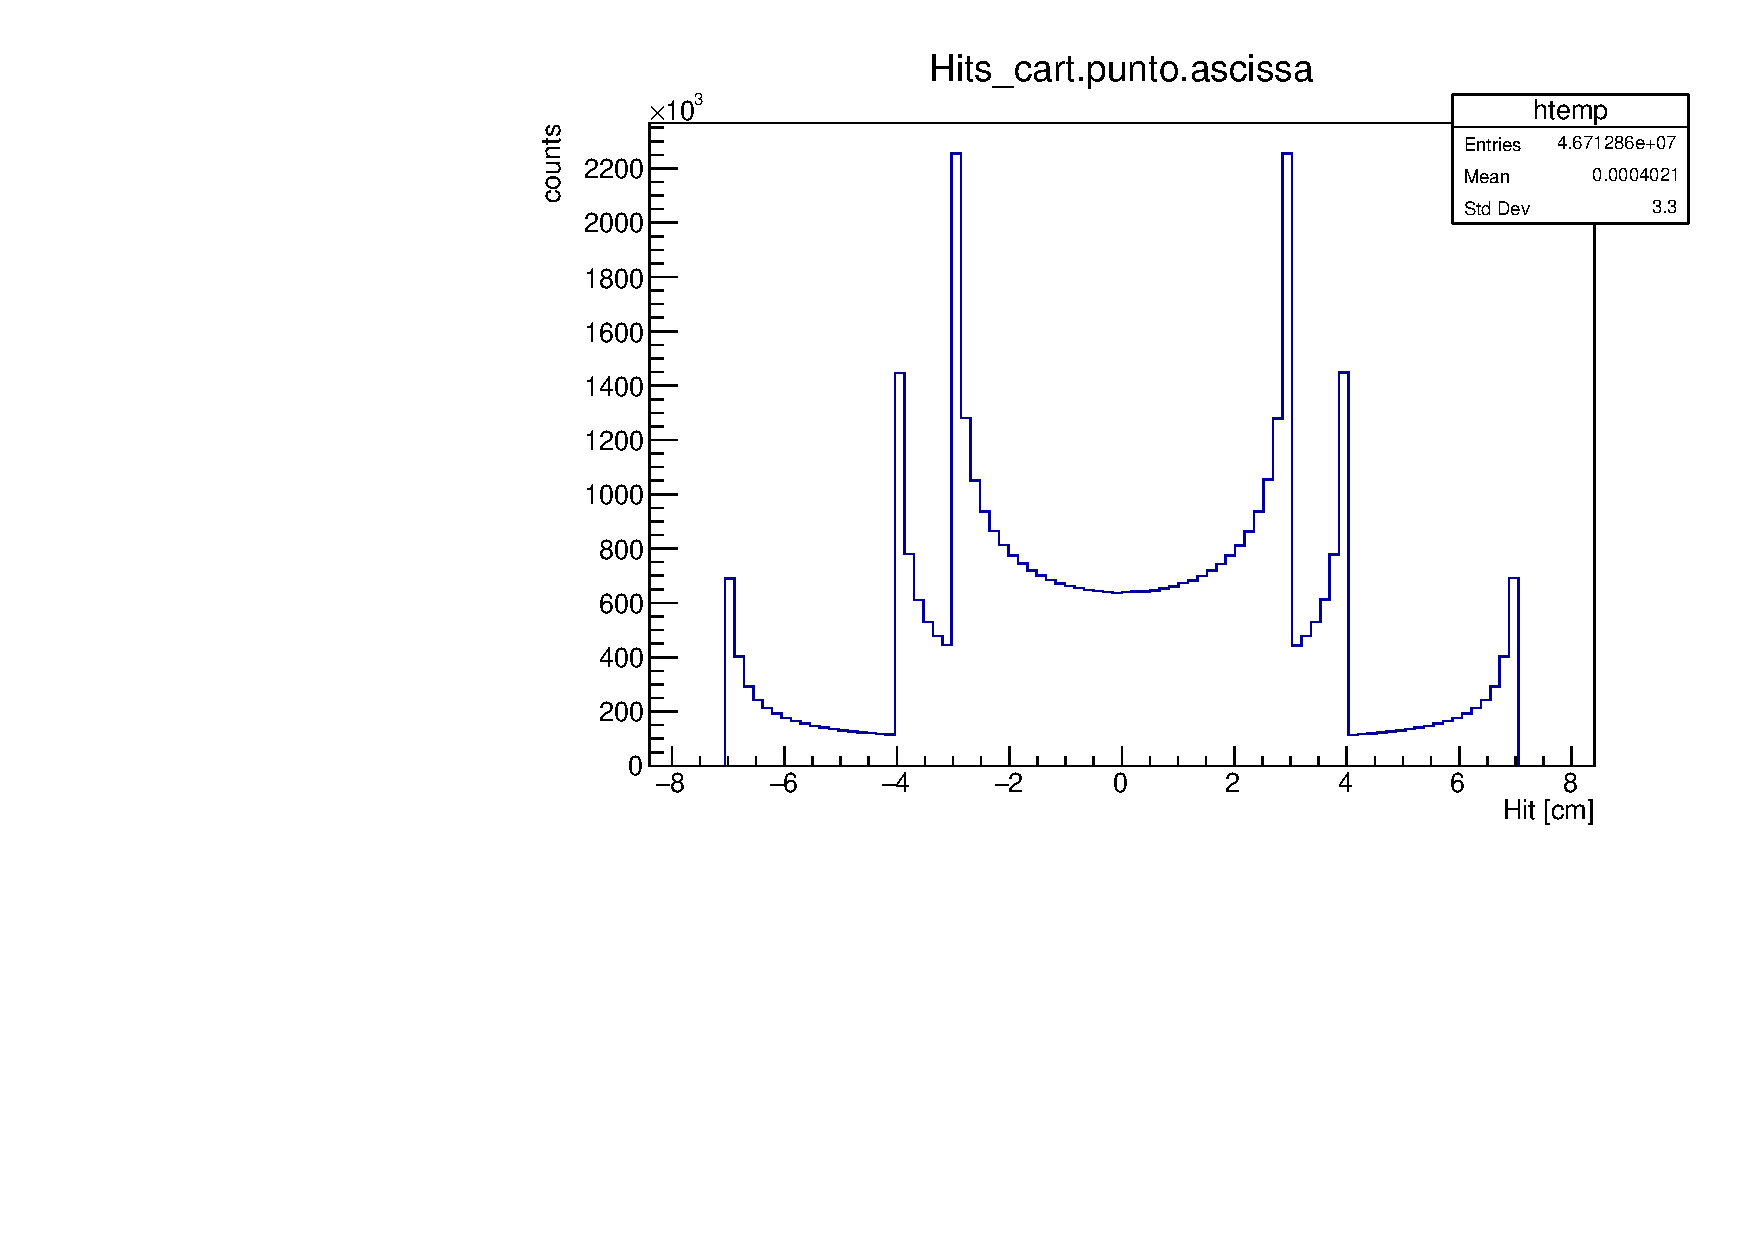
\includegraphics[width=0.3\textwidth]{images/S_x_tot.pdf}} 
    \subfigure[]{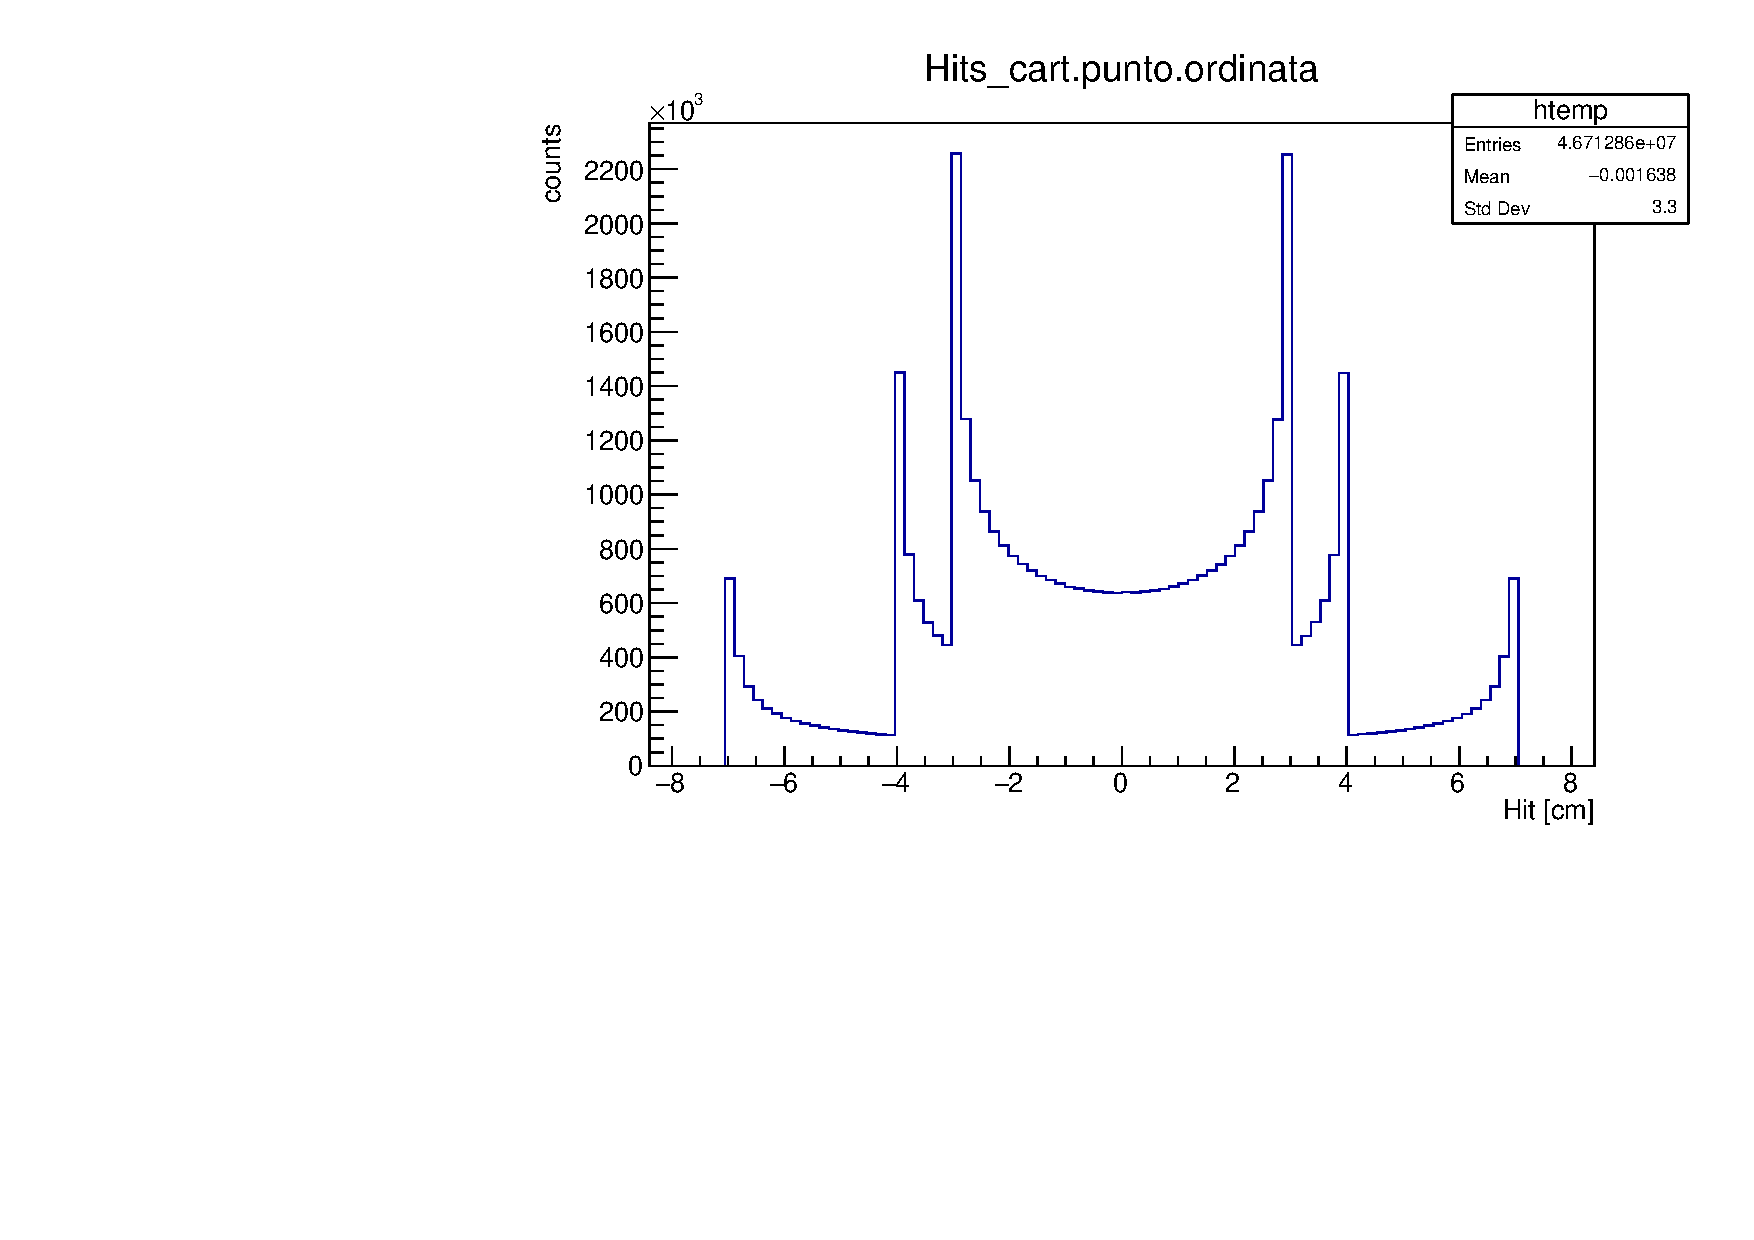
\includegraphics[width=0.3\textwidth]{images/S_y_tot.pdf}} 
    \subfigure[]{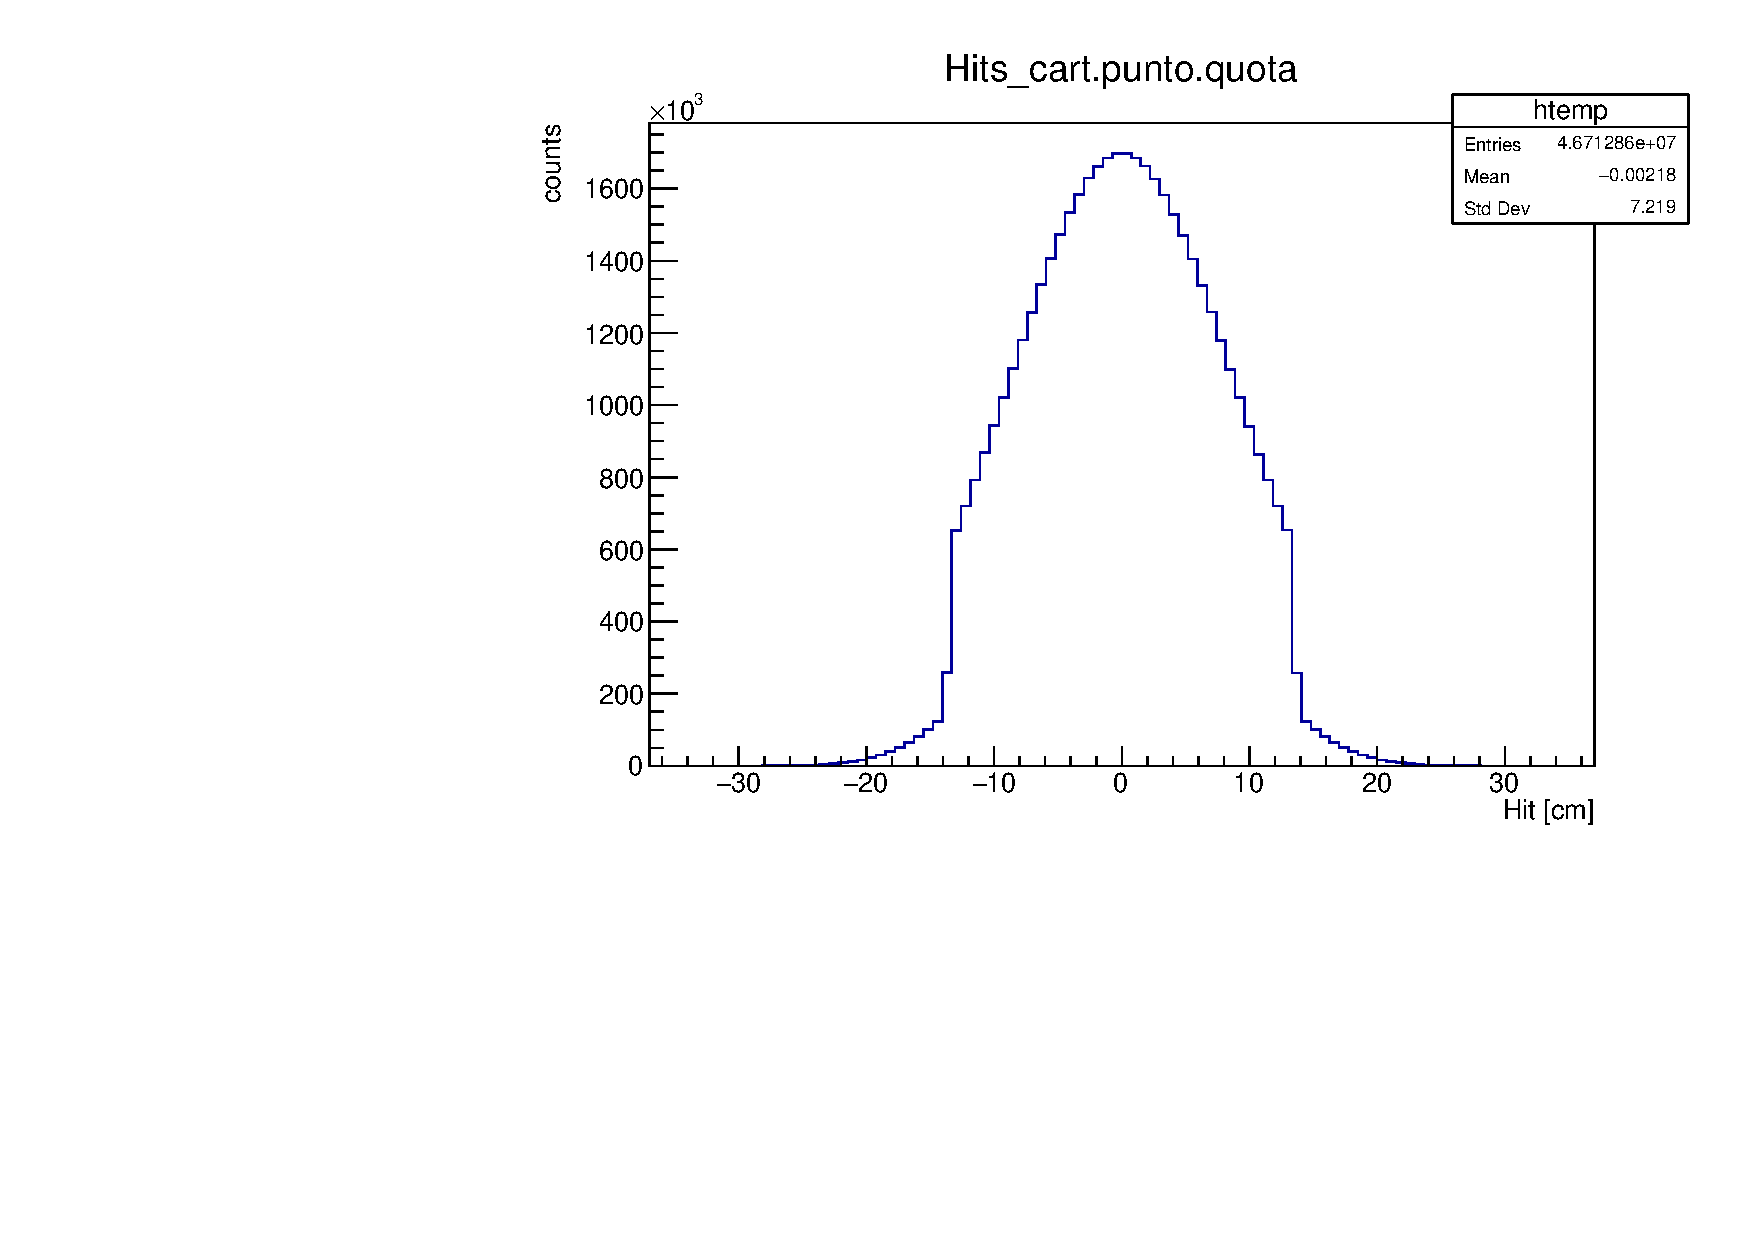
\includegraphics[width=0.3\textwidth]{images/S_z_tot.pdf}}
     \subfigure[]{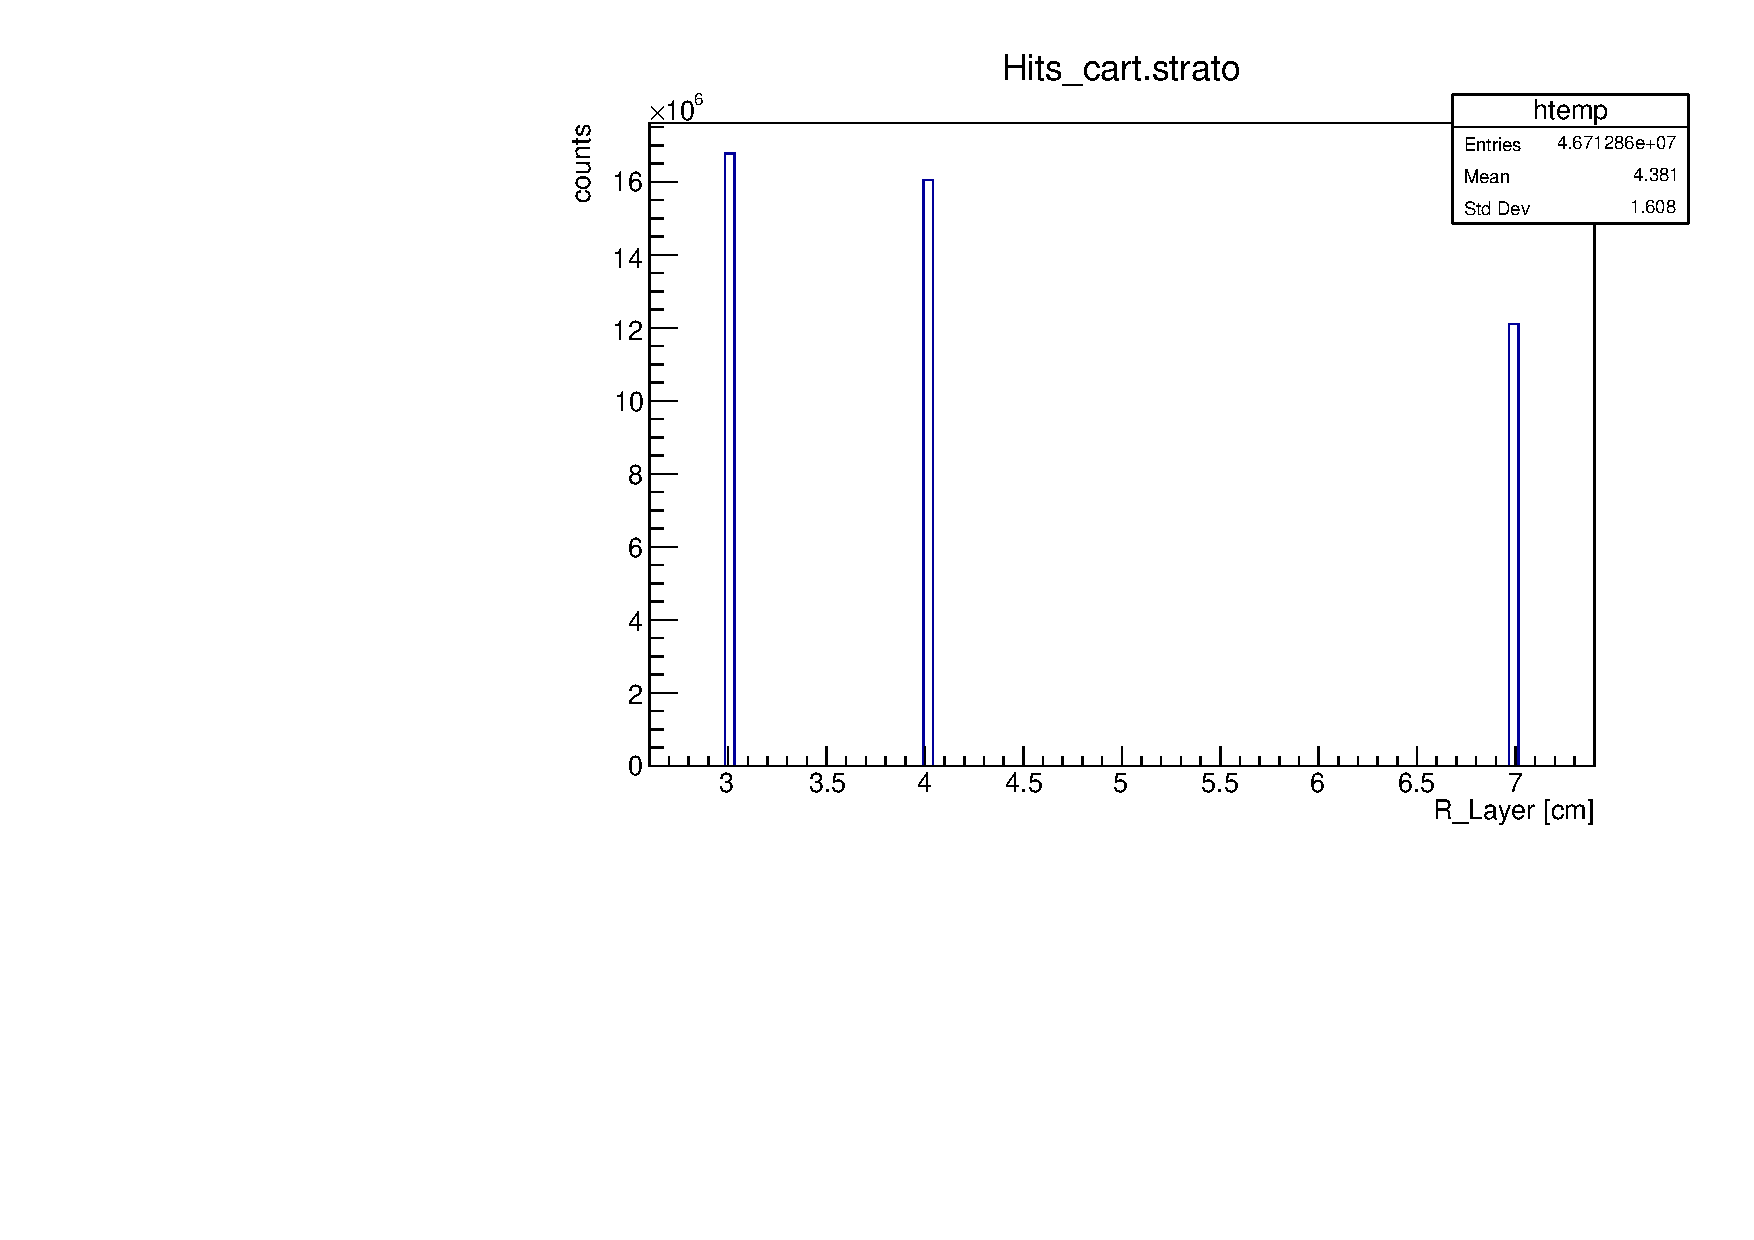
\includegraphics[width=0.55\textwidth]{images/S_layers.pdf}} 
    \caption{(a) asse x (b) asse y (c) asse z (d) hit sul raggio}
    
    \label{fig:foobar}
\end{figure}
Si può notare che anche la posizione sulla beam pipe viene contemplata, in quanto la realtà Monte Carlo rappresenta il puro evento fisico, estraneo al processo di rivelazione.
$\\$
Si riportano di seguito le caratteristiche del vertice d'interazione, in particolare la distribuzione della quota $Z_{true}$ e la distribuzione della molteplicità, che in questo esempio è quella assegnata ("hm"):

\begin{figure} [H]
    \centering
     \subfigure[]{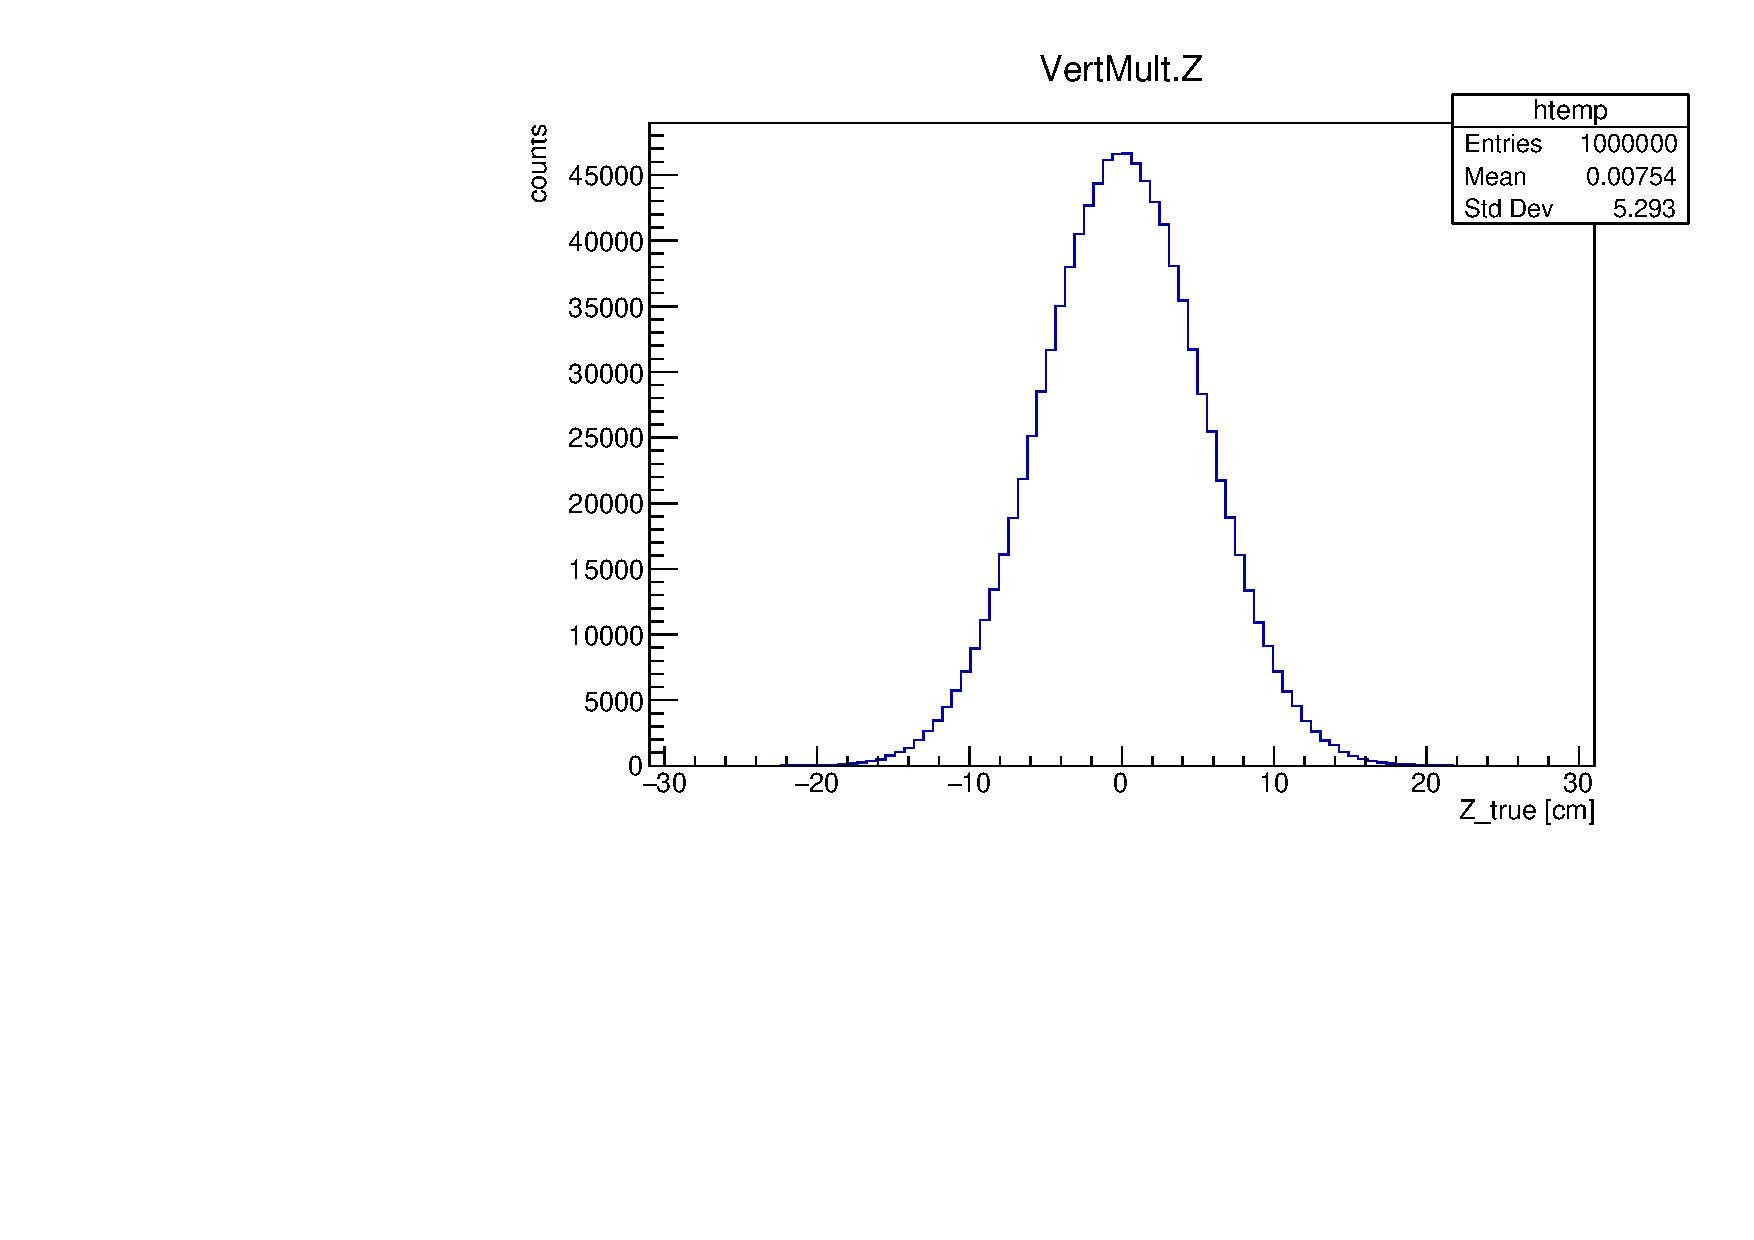
\includegraphics[width=0.45\textwidth]{images/S_z_true.pdf}} 
    \subfigure[]{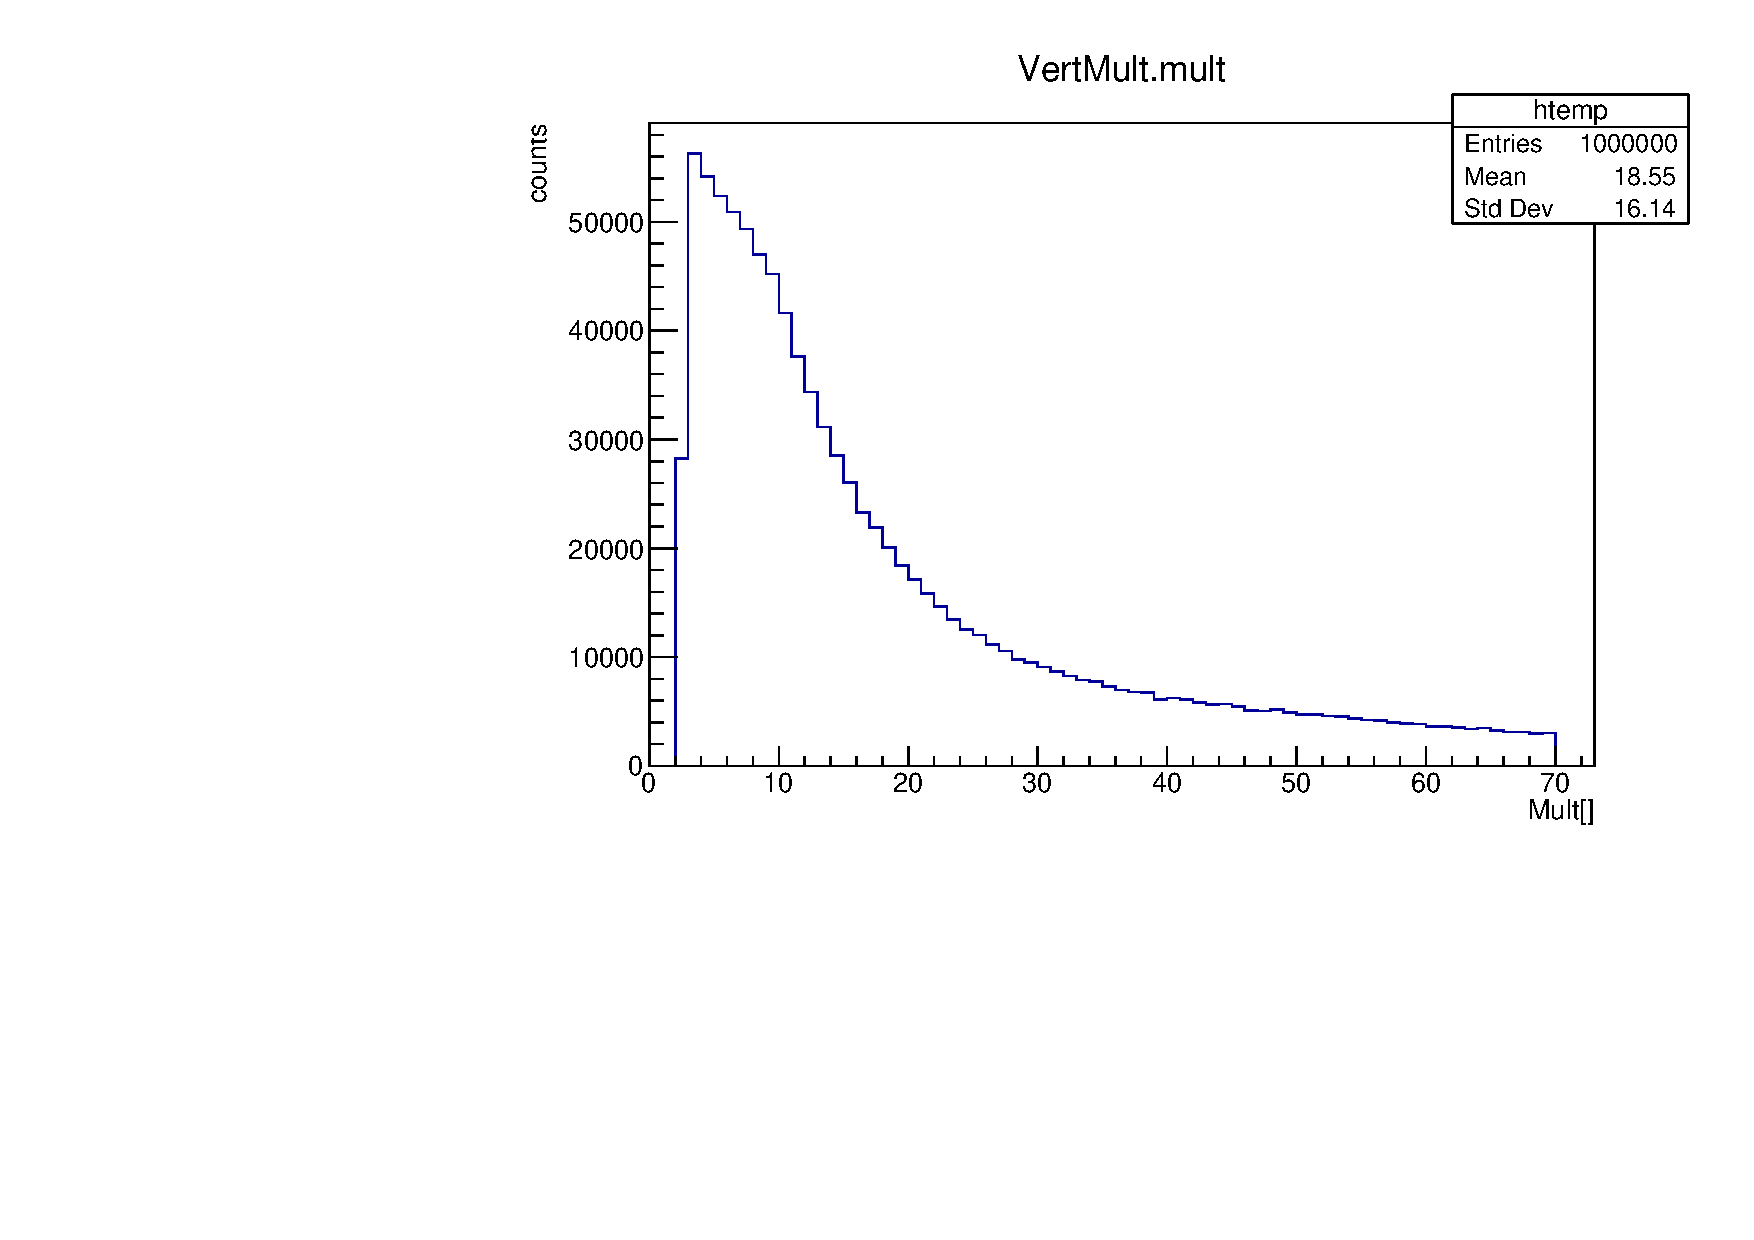
\includegraphics[width=0.45\textwidth]{images/S_mult.pdf}}
    \caption{(a) $Z_{true}$ (b) Molteplicità}
    
    \label{fig:foobar}
\end{figure}

\subsection {Rivelazione}
Dopo aver creato il processo fisico puro, si avvia il processo di rivelazione. Pertanto, si lancia la funzione dataReal\textunderscore TANS (bool spur, double noise). Questa ricrea il comportamento dei due layer in silicio, implementando anche la risposta in termini di risoluzione del rivelatore, attraverso un processo di smearing gaussiano. 
$\\$
Gli argomenti sono opzionabili affinché venga anche inscenata la presenza di rumore (spur = 1) o meno (spur = 0) e, nel primo caso, si può anche decidere, tunando opportunamente l'argomento noise, la quantità di rumore da iniettare. Se noise = 0, non si ha rumore. Se noise = 1, si è sommersi totalmente dal rumore. Si riportano di seguito le precedenti e medesime grandezze : 

\begin{figure} [H]
    \centering
    \subfigure[]{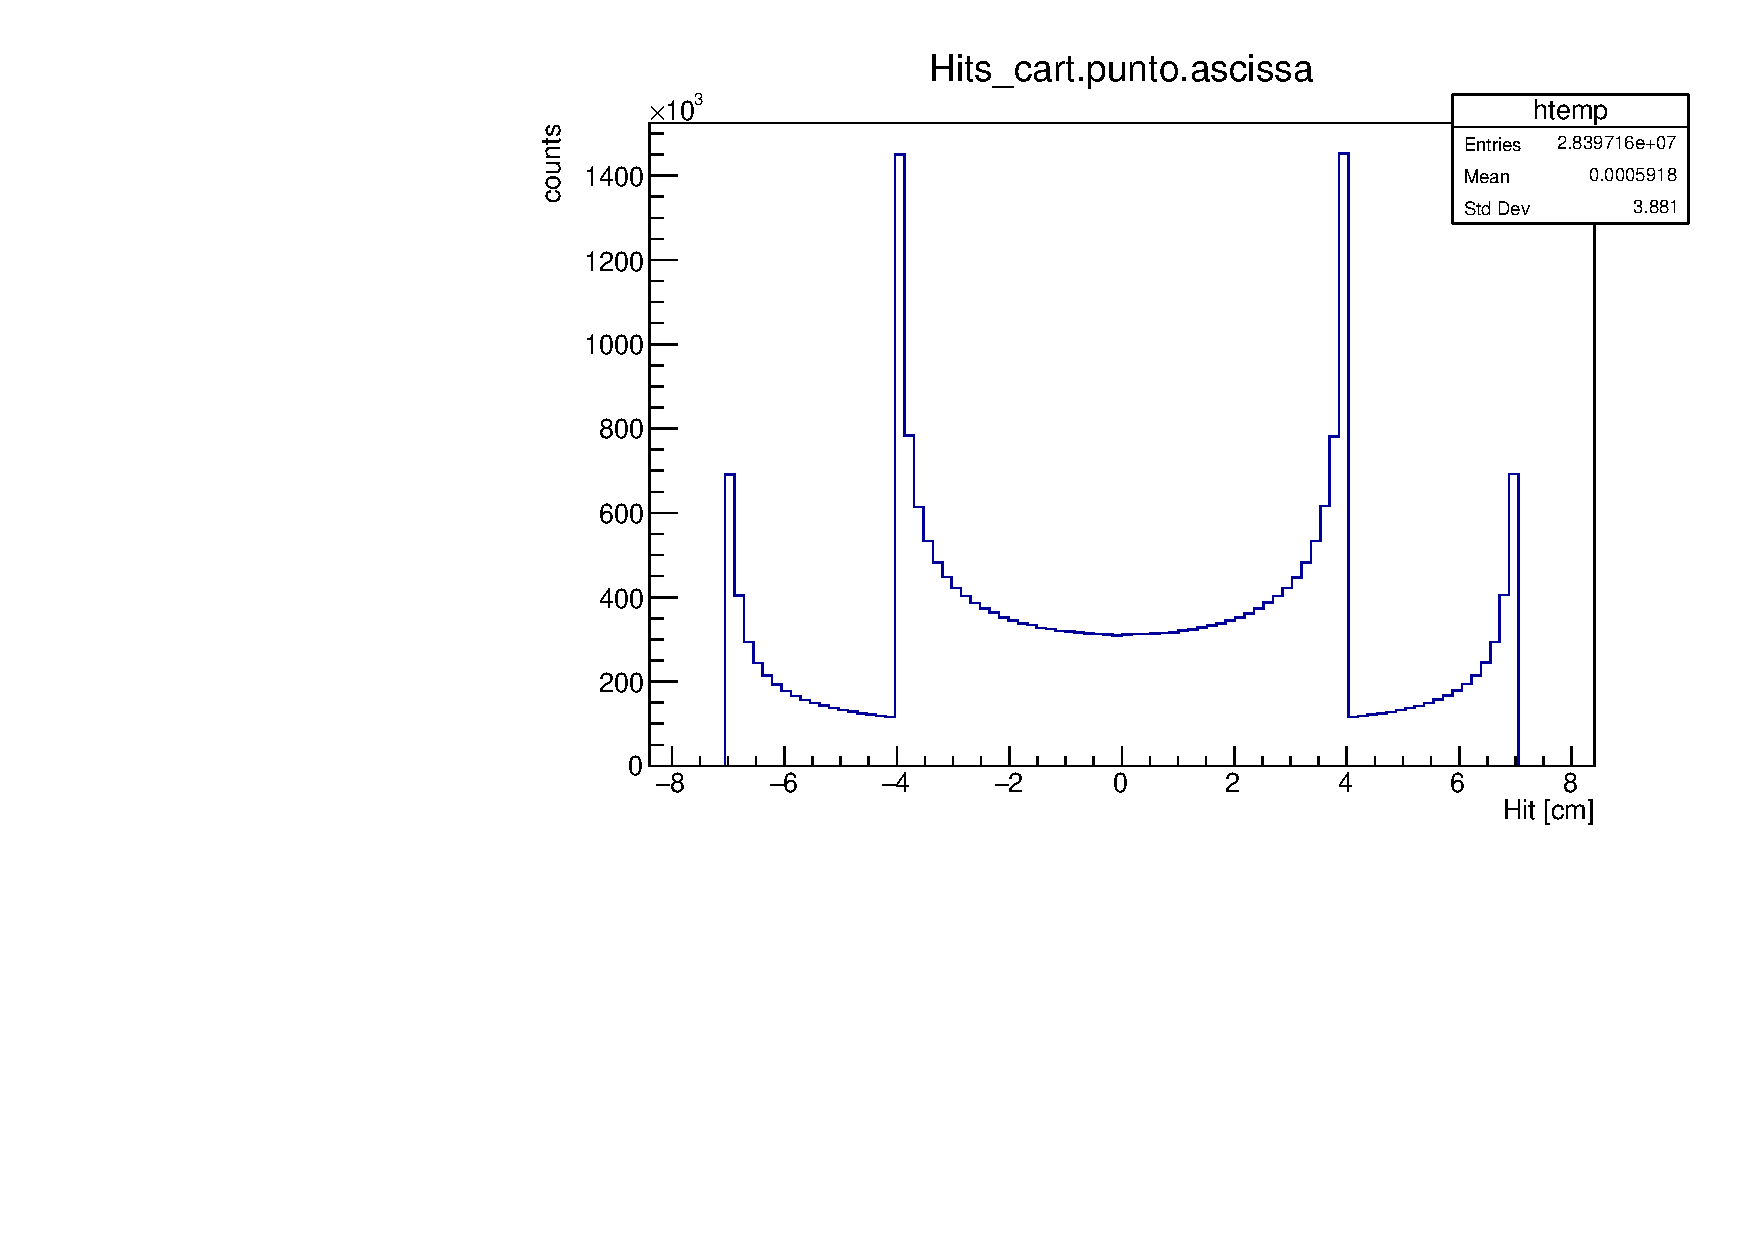
\includegraphics[width=0.3\textwidth]{images/D_x_tot.pdf}} 
    \subfigure[]{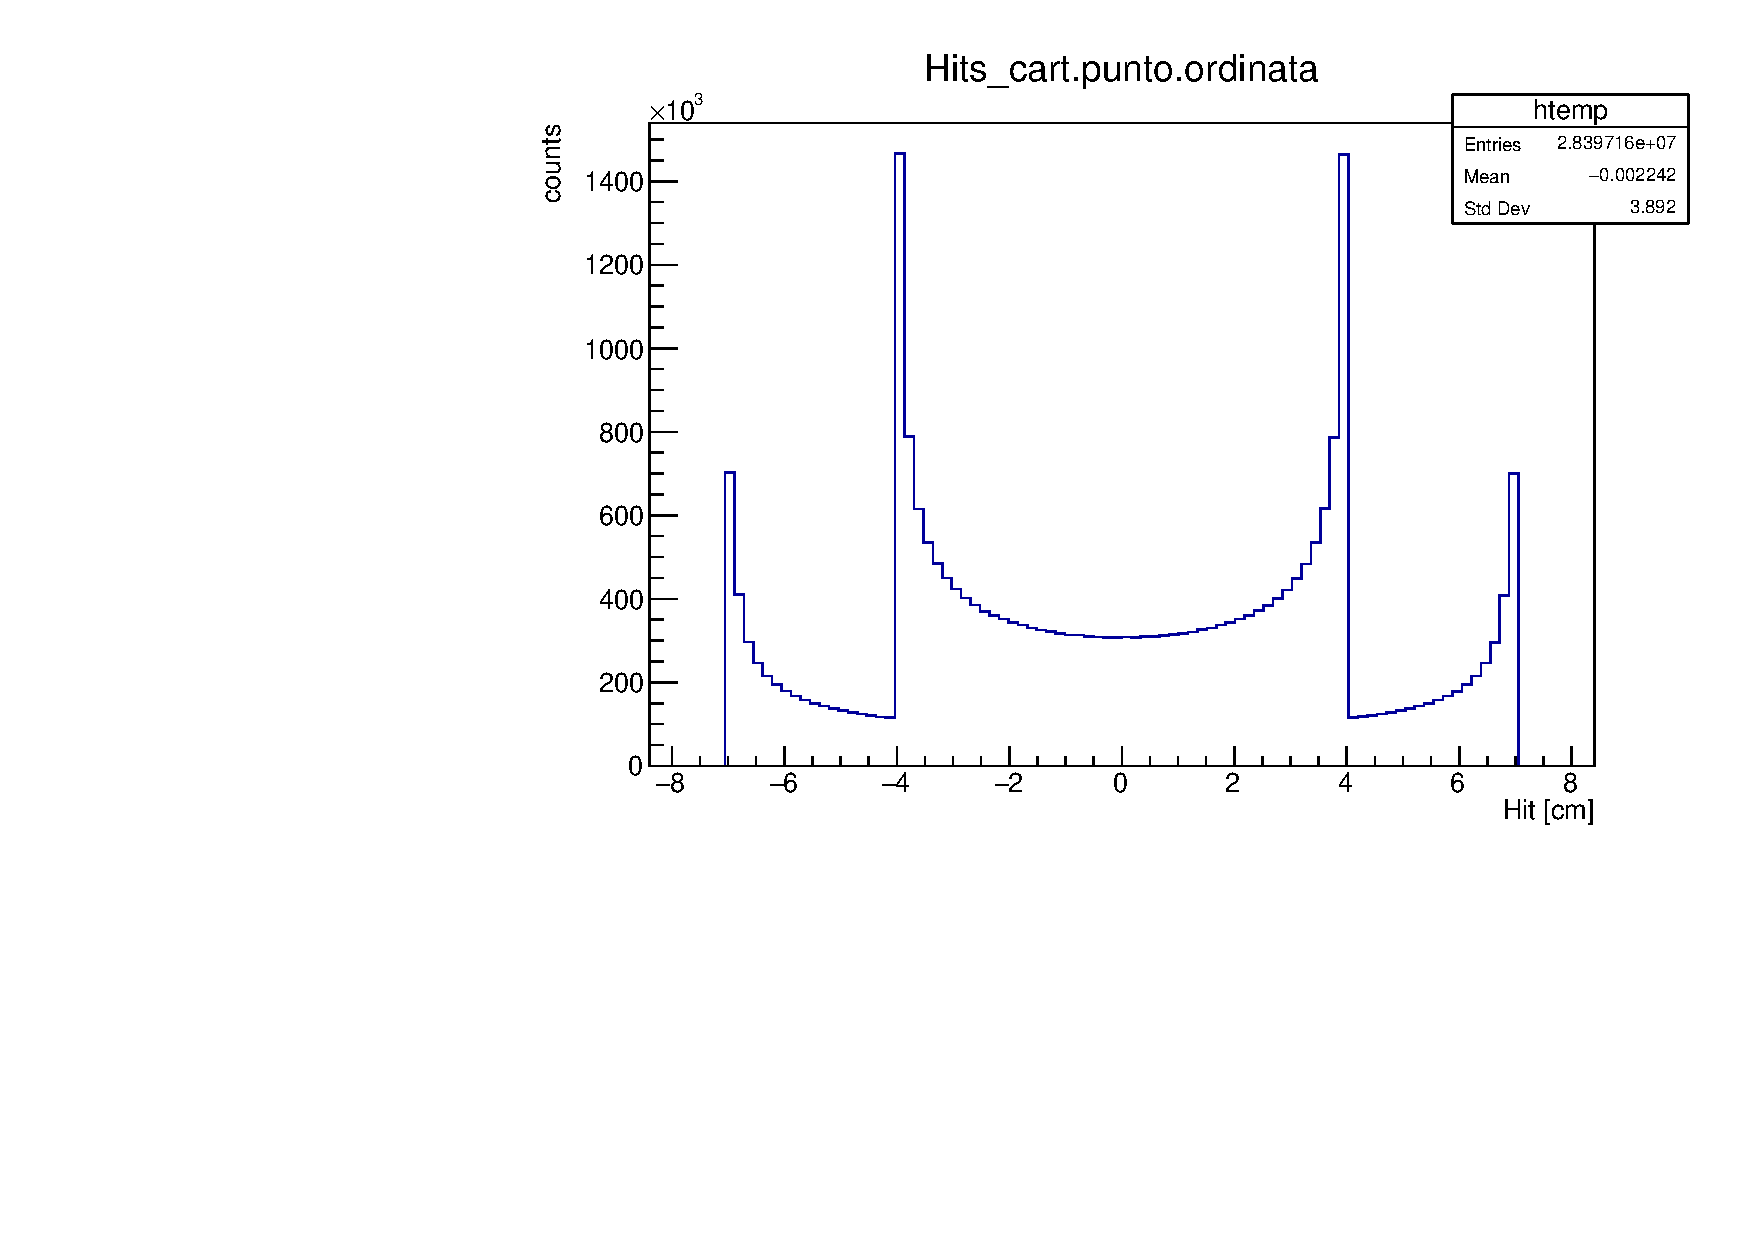
\includegraphics[width=0.3\textwidth]{images/D_y_tot.pdf}} 
    \subfigure[]{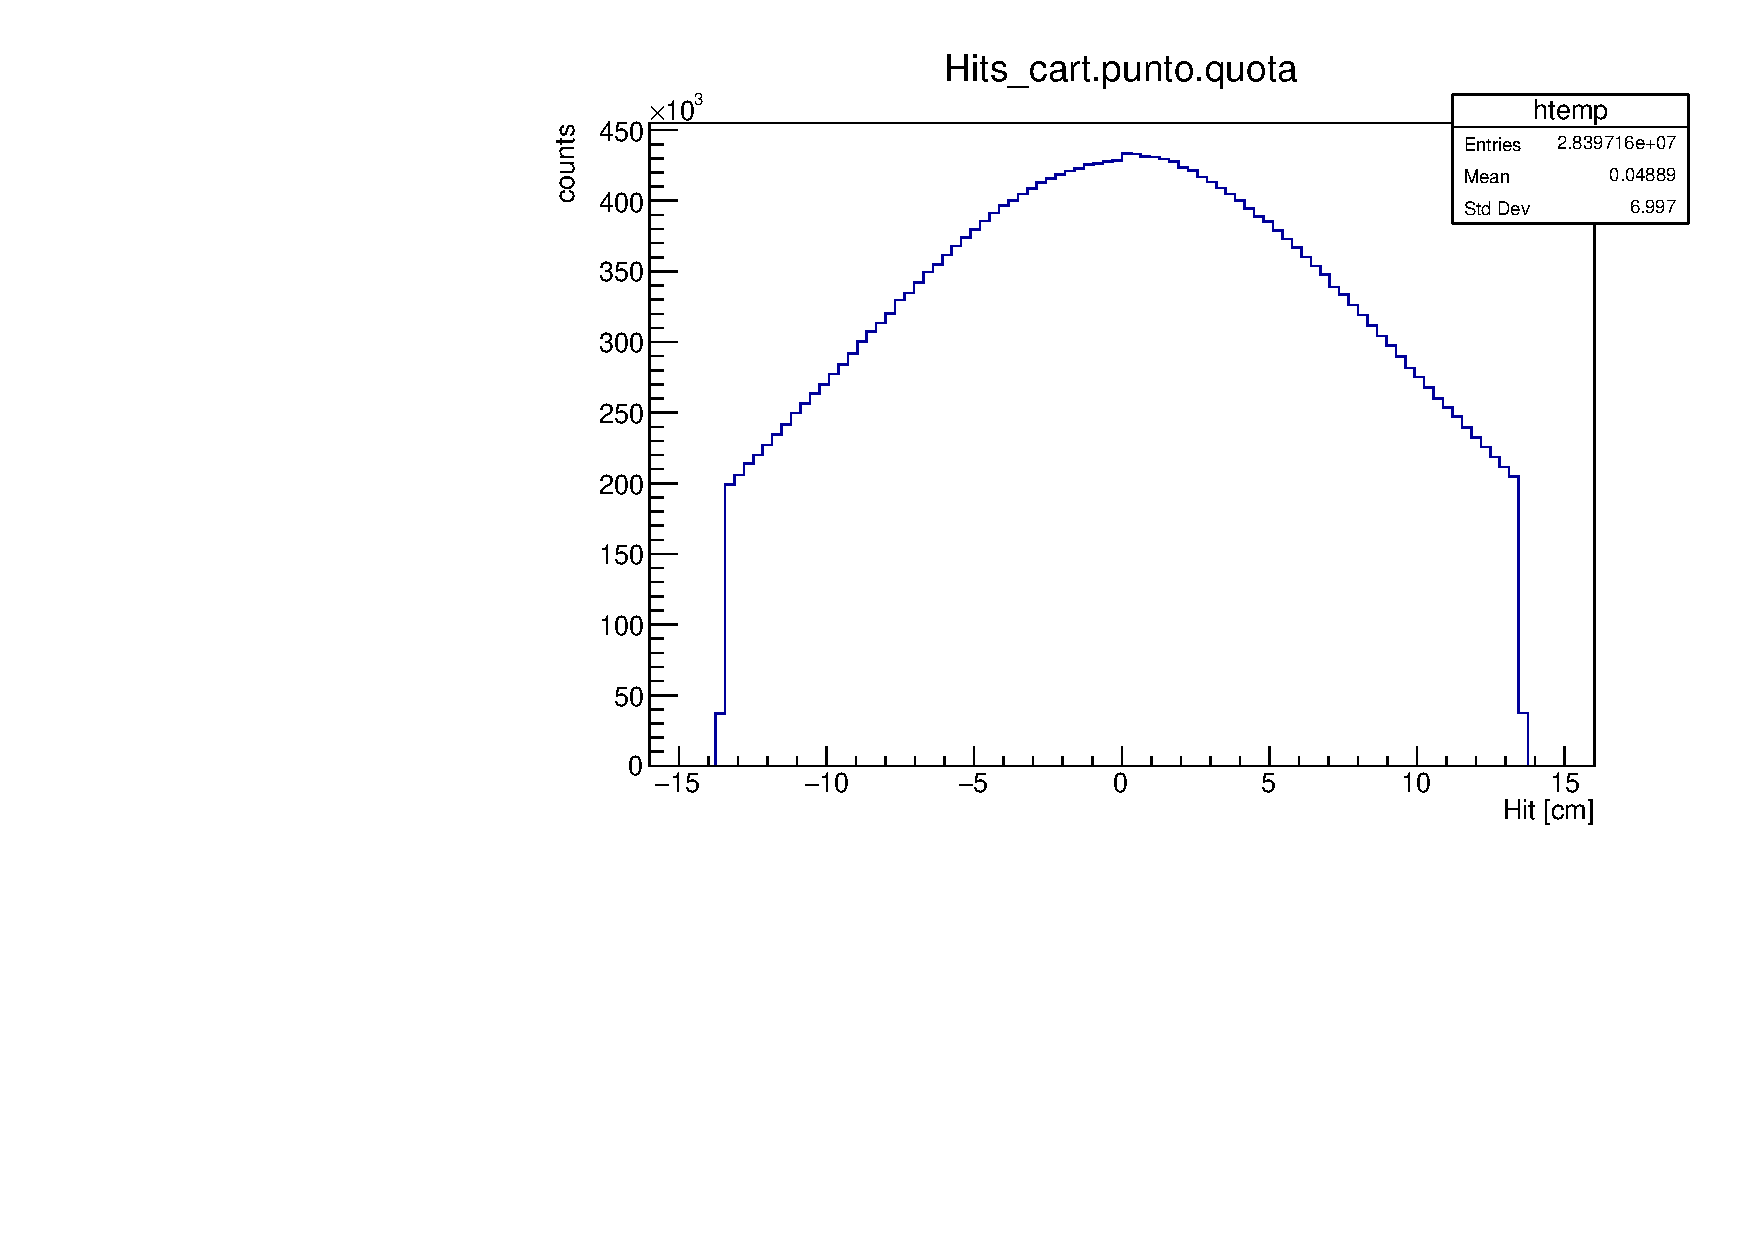
\includegraphics[width=0.3\textwidth]{images/D_z_tot.pdf}}
        \subfigure[]{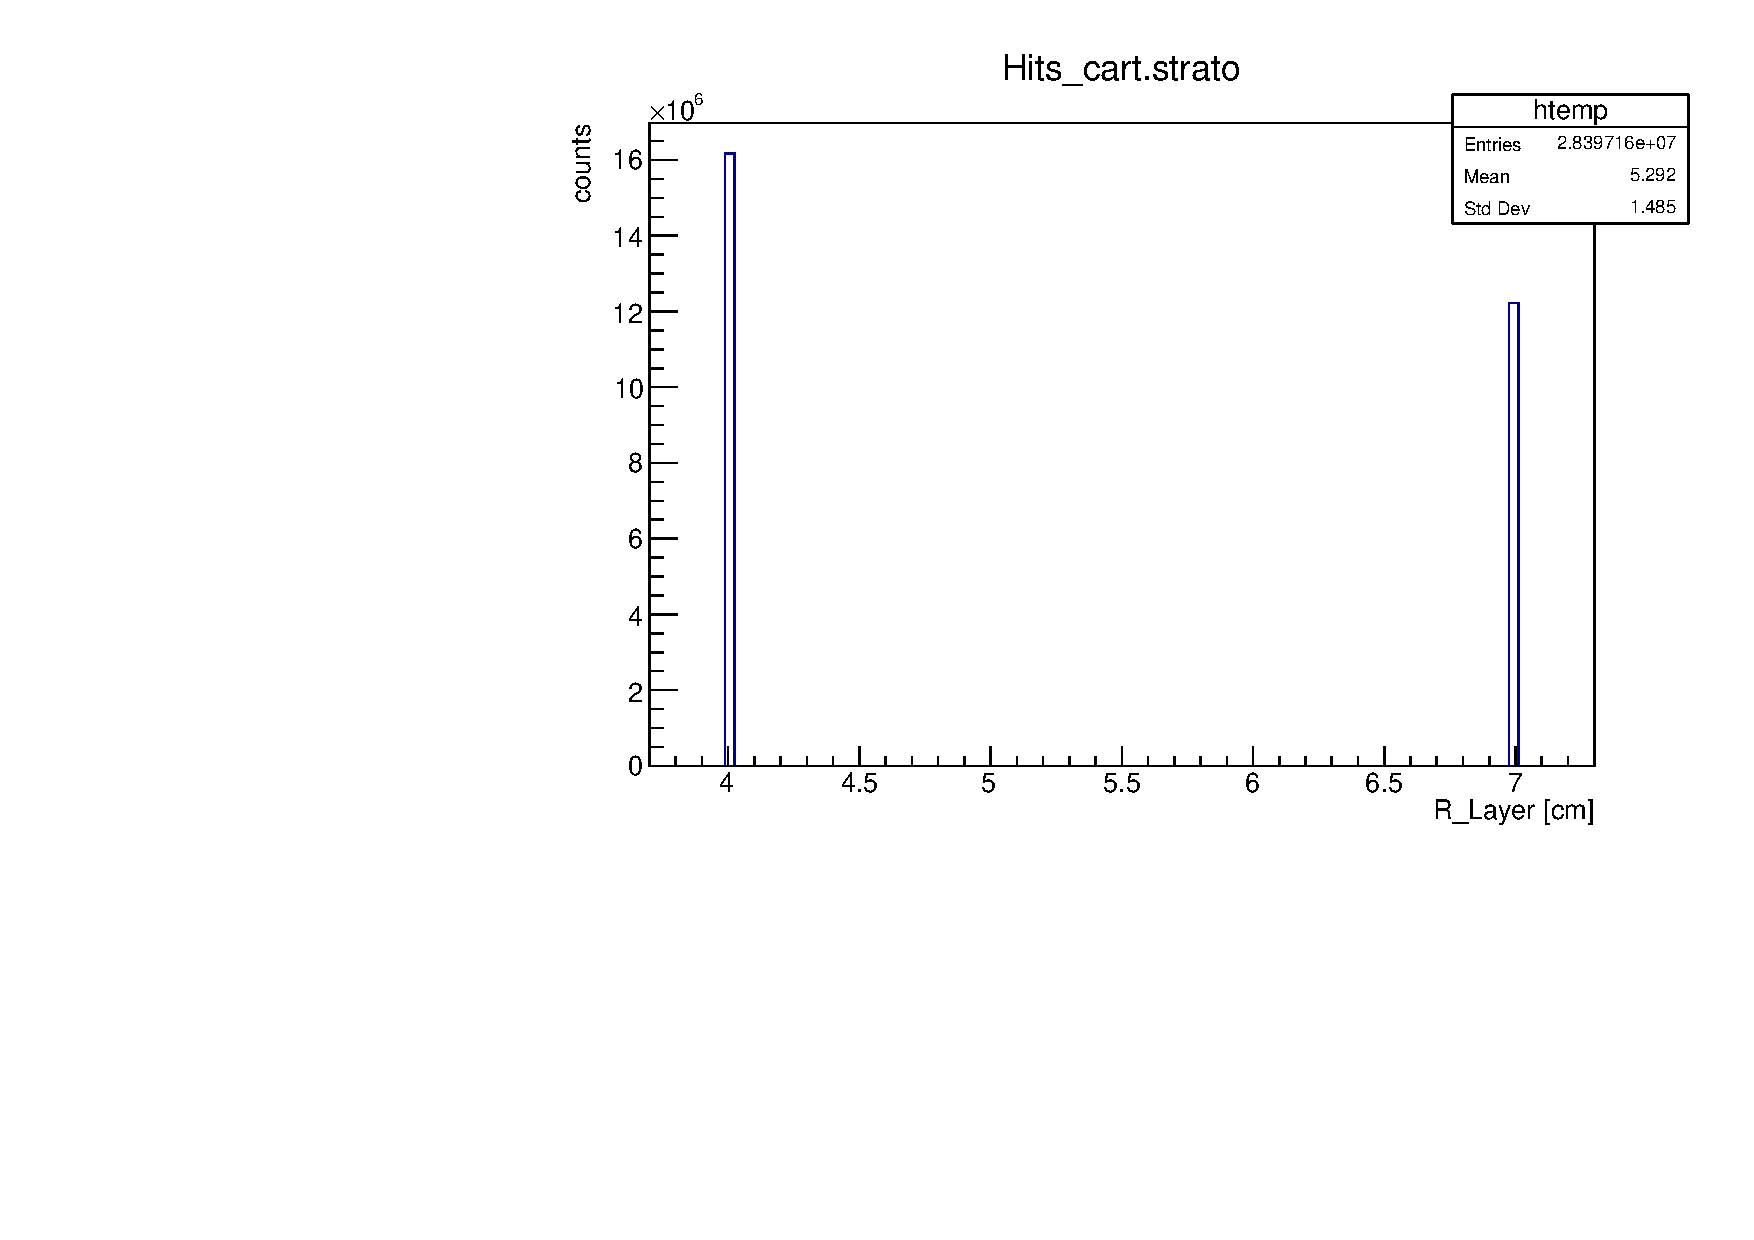
\includegraphics[width=0.55\textwidth]{images/D_layers.pdf}} 
    \caption{(a) asse x (b) asse y (c) asse z (d) hit sul raggio}
    \label{fig:foobar}
\end{figure}

Diversamente da prima, adesso viene evidenziato il comportamento attivo dei layers in silicio rispetto alla beam pipe, come si può notare.
$\\$
Viene creato il file "data.root", che rappresenta il pool di dati simulato a seguito della rivelazione. Al suo interno vi sono gli hit sui layer 2 e 3, che corrispondono ai rivelatori. Questo è il dataset reale, ovvero quello che ci si aspetta di ottenere a seguito di una presa dati. 

\subsection{Ricostruzione}
Si avvia un processo di ricostruzione del vertice di questi dati simulati presenti sul file "data.root", chiamando la funzione ricostruz\textunderscore TANS(double window), che si incarica di prendere gli oggetti creati dalla rivelazione e di determinare la posizione del vertice evento per evento, salvando tutto nel file "ricostruz.root". Si può scegliere quanto essere "elastici" nella restrizione del dataset z\textunderscore rec attraverso la scelta di window, che modula la rispettiva finestra di taglio in unità di $\sigma_z$. Di seguito si riporta la distribuzione della quota ricostruita relativa al vertice d'interazione $Z_{rec}$:

\begin{center}
    	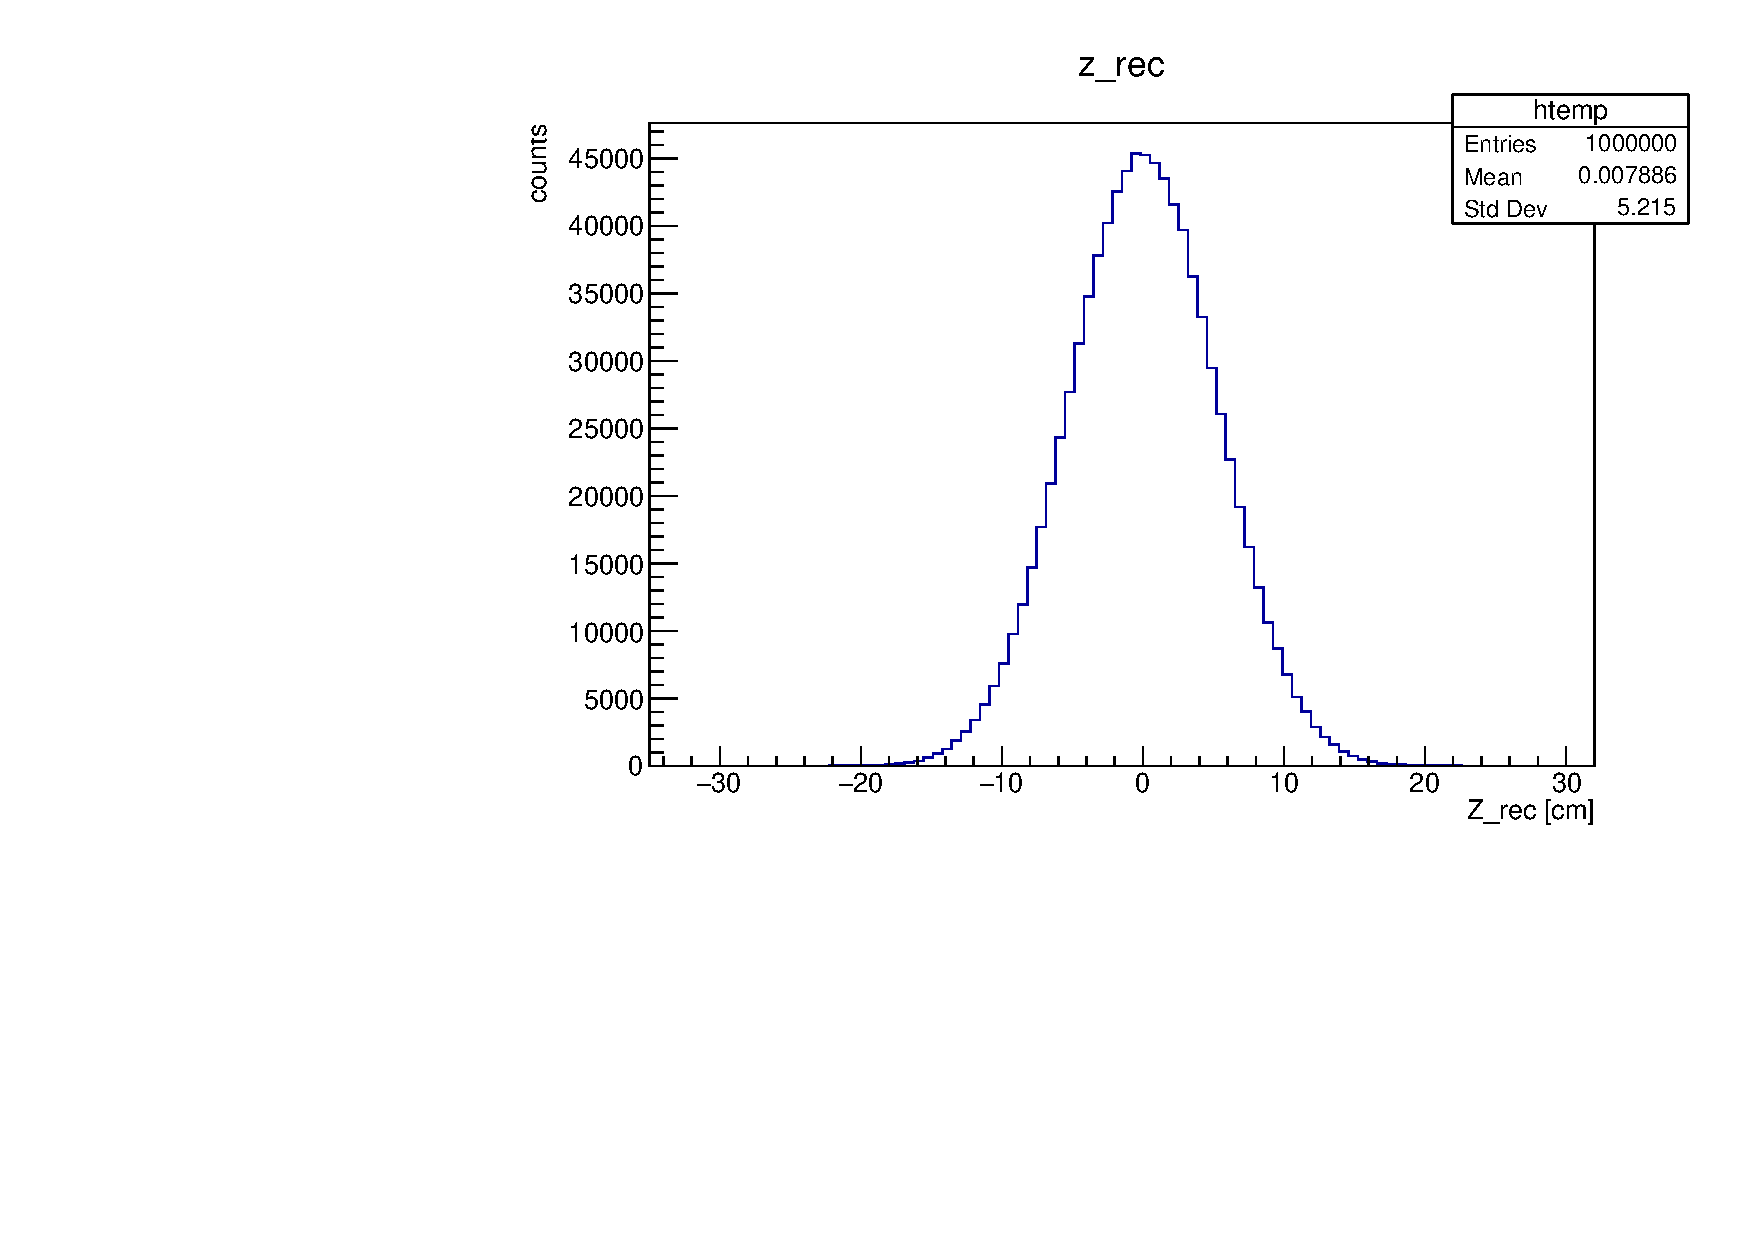
\includegraphics[width=0.55\linewidth]{images/R_z_rec.pdf}
\end{center}

\subsection{Residui tra $Z_{true}$ e $Z_{rec}$}
Si lancia la funzione " residues\textunderscore TANS () " che preleva Z\textunderscore true e Z\textunderscore rec dai rispettivi TTree e ne produce il residuo. Si evidenzia il fatto che quest'ultimo è relativo alla distribuzione scelta in partenza, quindi comprende tutti i contributi in termini di molteplicità e restituisce una distribuzione che è, in generale, non gaussiana:
\begin{center}
    	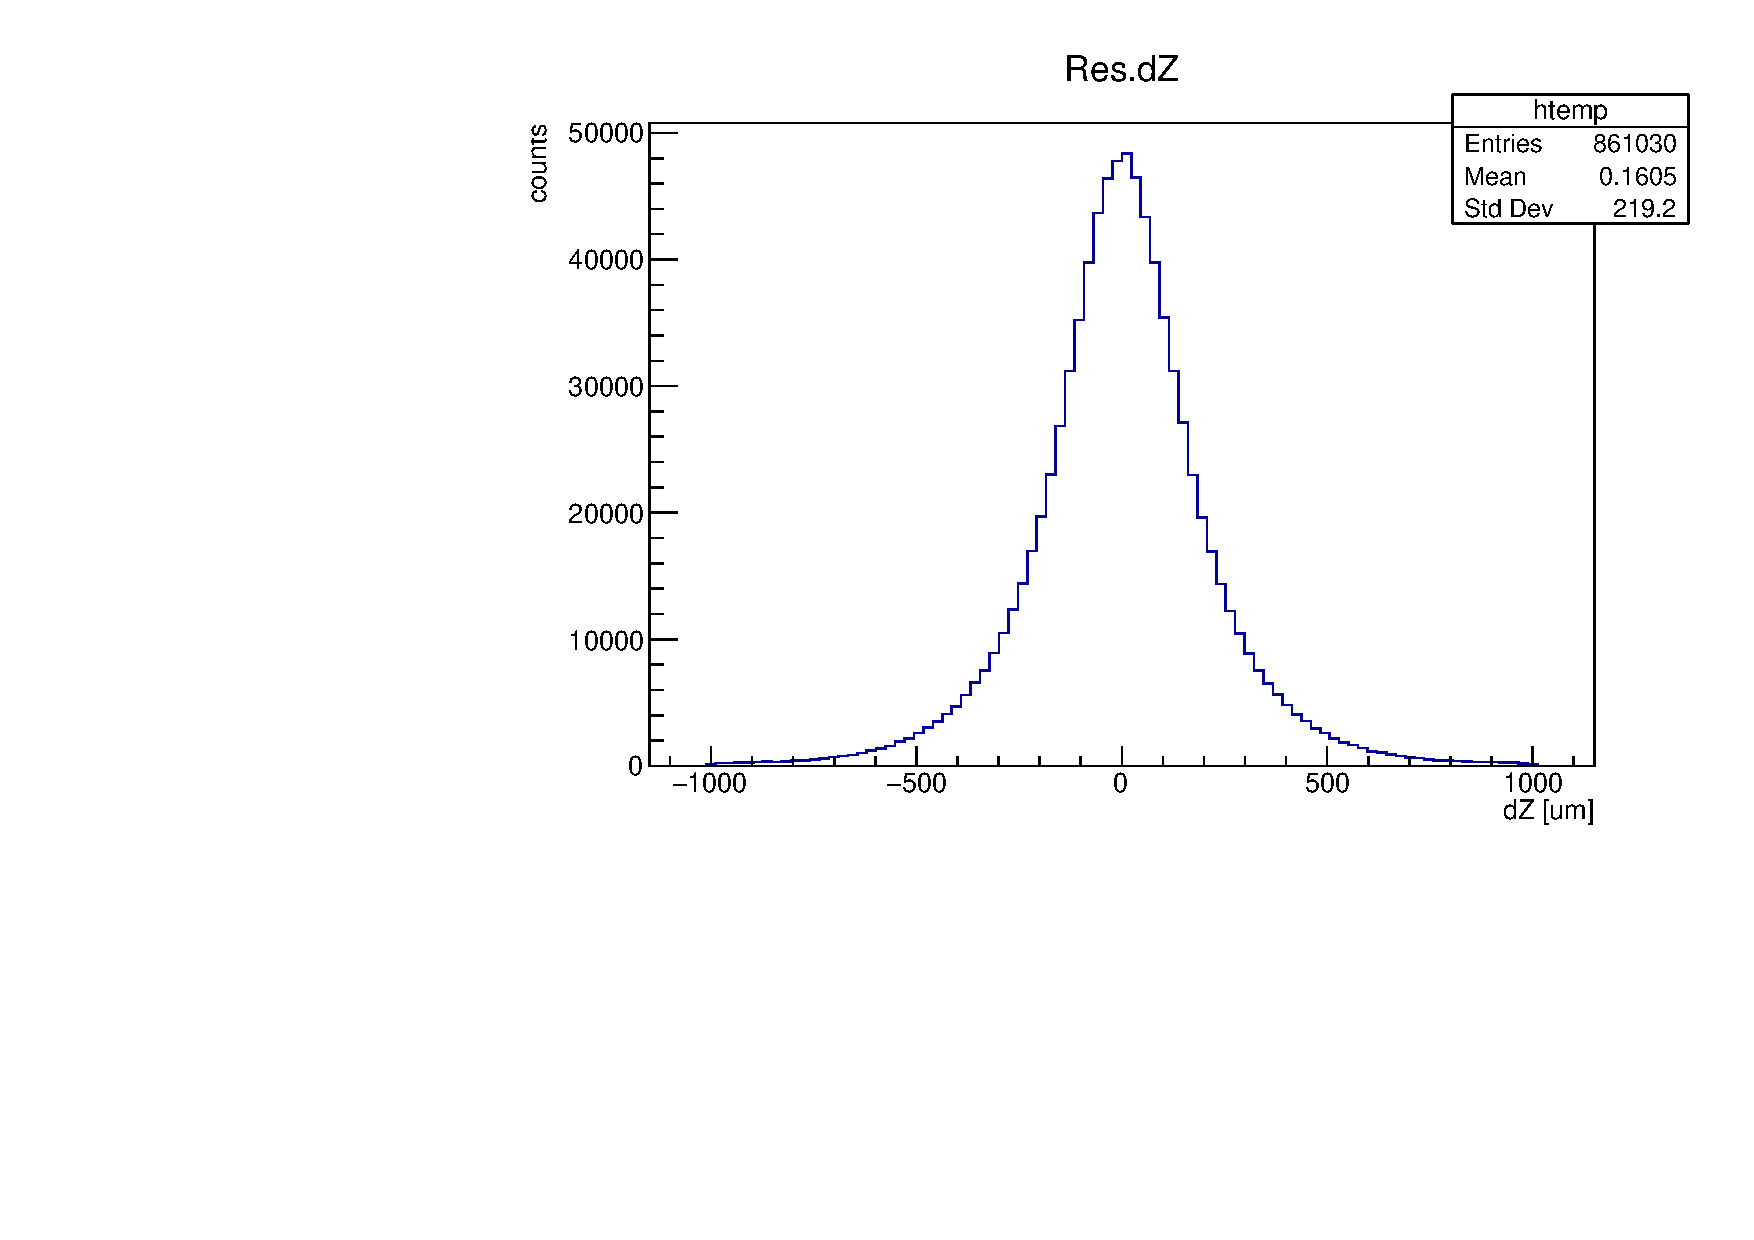
\includegraphics[width=0.65\linewidth]{images/res_dz.pdf}
\end{center}

Le distribuzioni gaussiane relative ai vari tagli di molteplicità vengono presentate nel sezione 4. 


\subsection{Event display}
Si lancia la funzione "TGeo\textunderscore personal(int ev)", che si incarica di svolgere un event display (molto rudimentale) della realtà Monte Carlo e che come argomento ha il numero dell'evento che si vuole rappresentare. Viene ristampato il risultato finale, ossia il Z\textunderscore true e Z\textunderscore rec. 
Per una miglior interfaccia, si consiglia di utilizzare un 3D Viewer quale OpenGL, selezionabile direttamente dal TCanvas in uscita. L'interfaccia che si presenta è la seguente:
\begin{figure} [H]
    \centering
    \subfigure[]{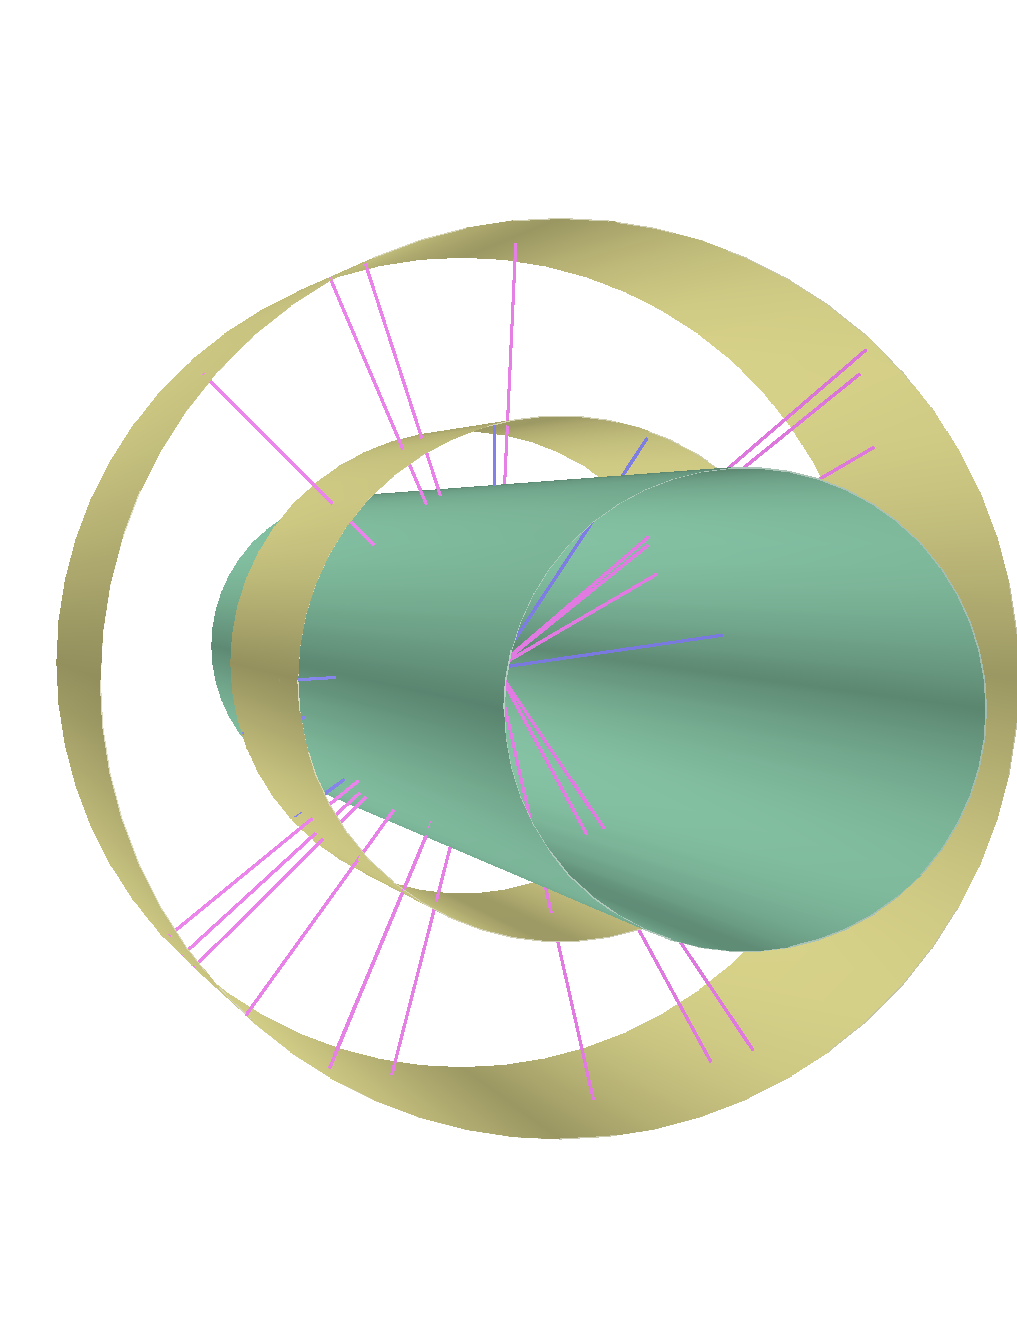
\includegraphics[width=0.4\textwidth]{images/3D_ev.pdf}} 
    \subfigure[]{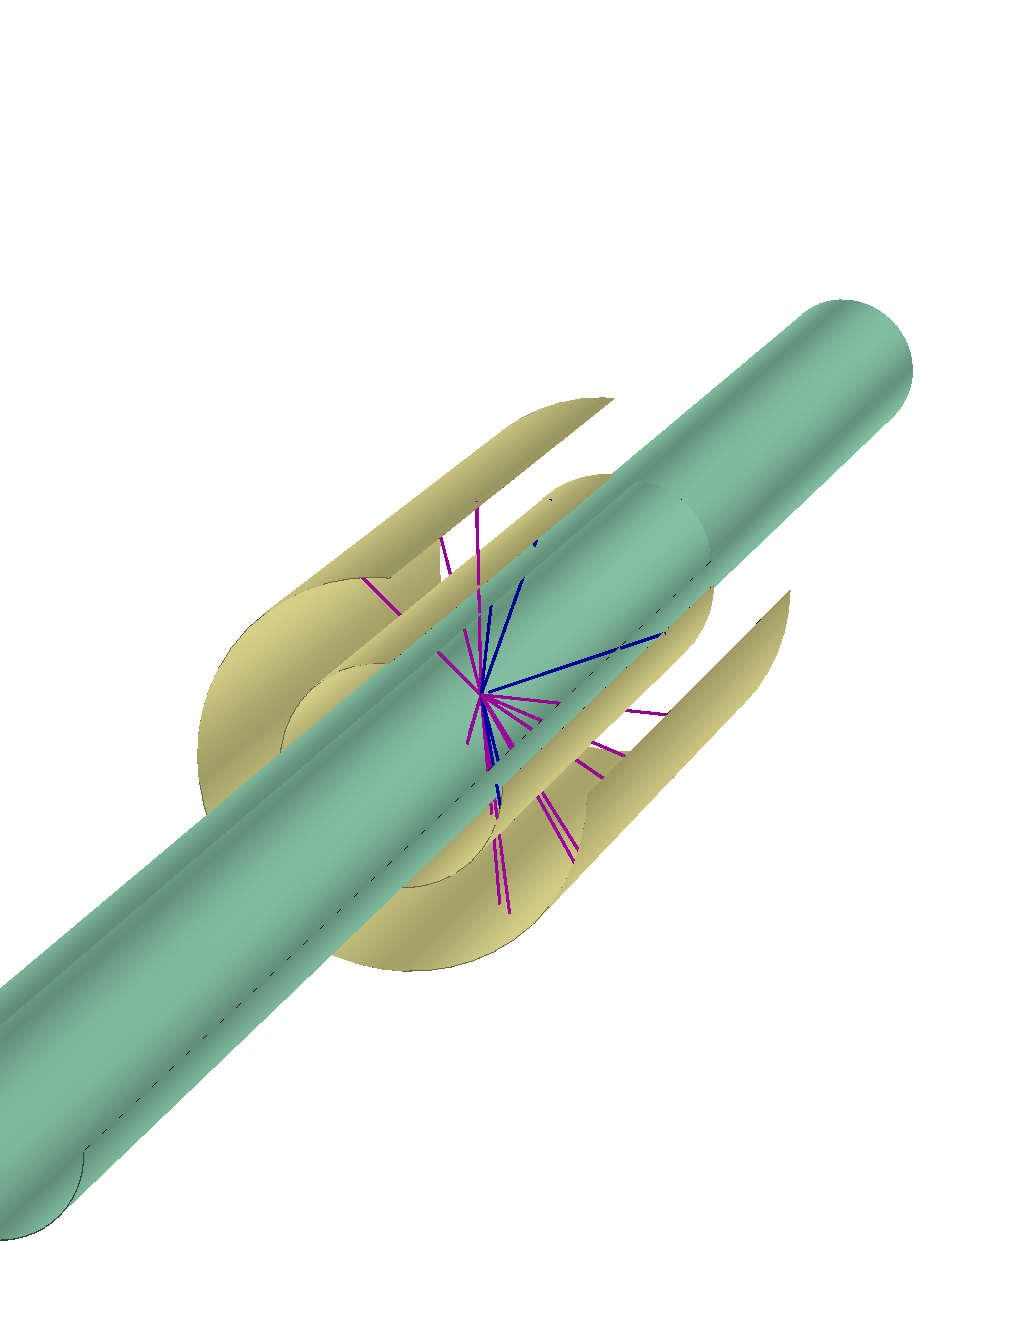
\includegraphics[width=0.4\textwidth]{images/sec_3D_ev.pdf}} 
    \caption{(a) evento d'esempio (b) sezione dell'evento d'esempio}
    \label{fig:foobar}
\end{figure}

\section {Performance}
Si intende adesso fornire un andamento della risoluzione e dell'efficienza, in relazione alla molteplicità e a $Z_{true}$. A tal fine, ci si colloca all'interno della directory "results\textunderscore TANS" e si interpreta la macro  comp\textunderscore TANS.C.

\subsection{Residui e molteplicità}
Si lancia la funzione "all\textunderscore residues()". Essa preleva l'istogramma dei residui e si incarica di rappresentare l'andamento del residuo "dZ", al variare della molteplicità selezionata attraverso dei tagli sulla variabile "mul" applicati direttamente al sovrastante istogramma dei residui. I risultati vengono salvati nel TTree presente in "residues.root".
$\\$
In questo contesto, dZ riceve un unico contributo in termini di molteplicità e, pertanto, si distribuisce secondo una gaussiana.
Si riportano di seguiti i risultati ottenuti, per un sottoinsieme di molteplicità selezionate:

\begin{figure} [H]
    \centering
    \subfigure[]{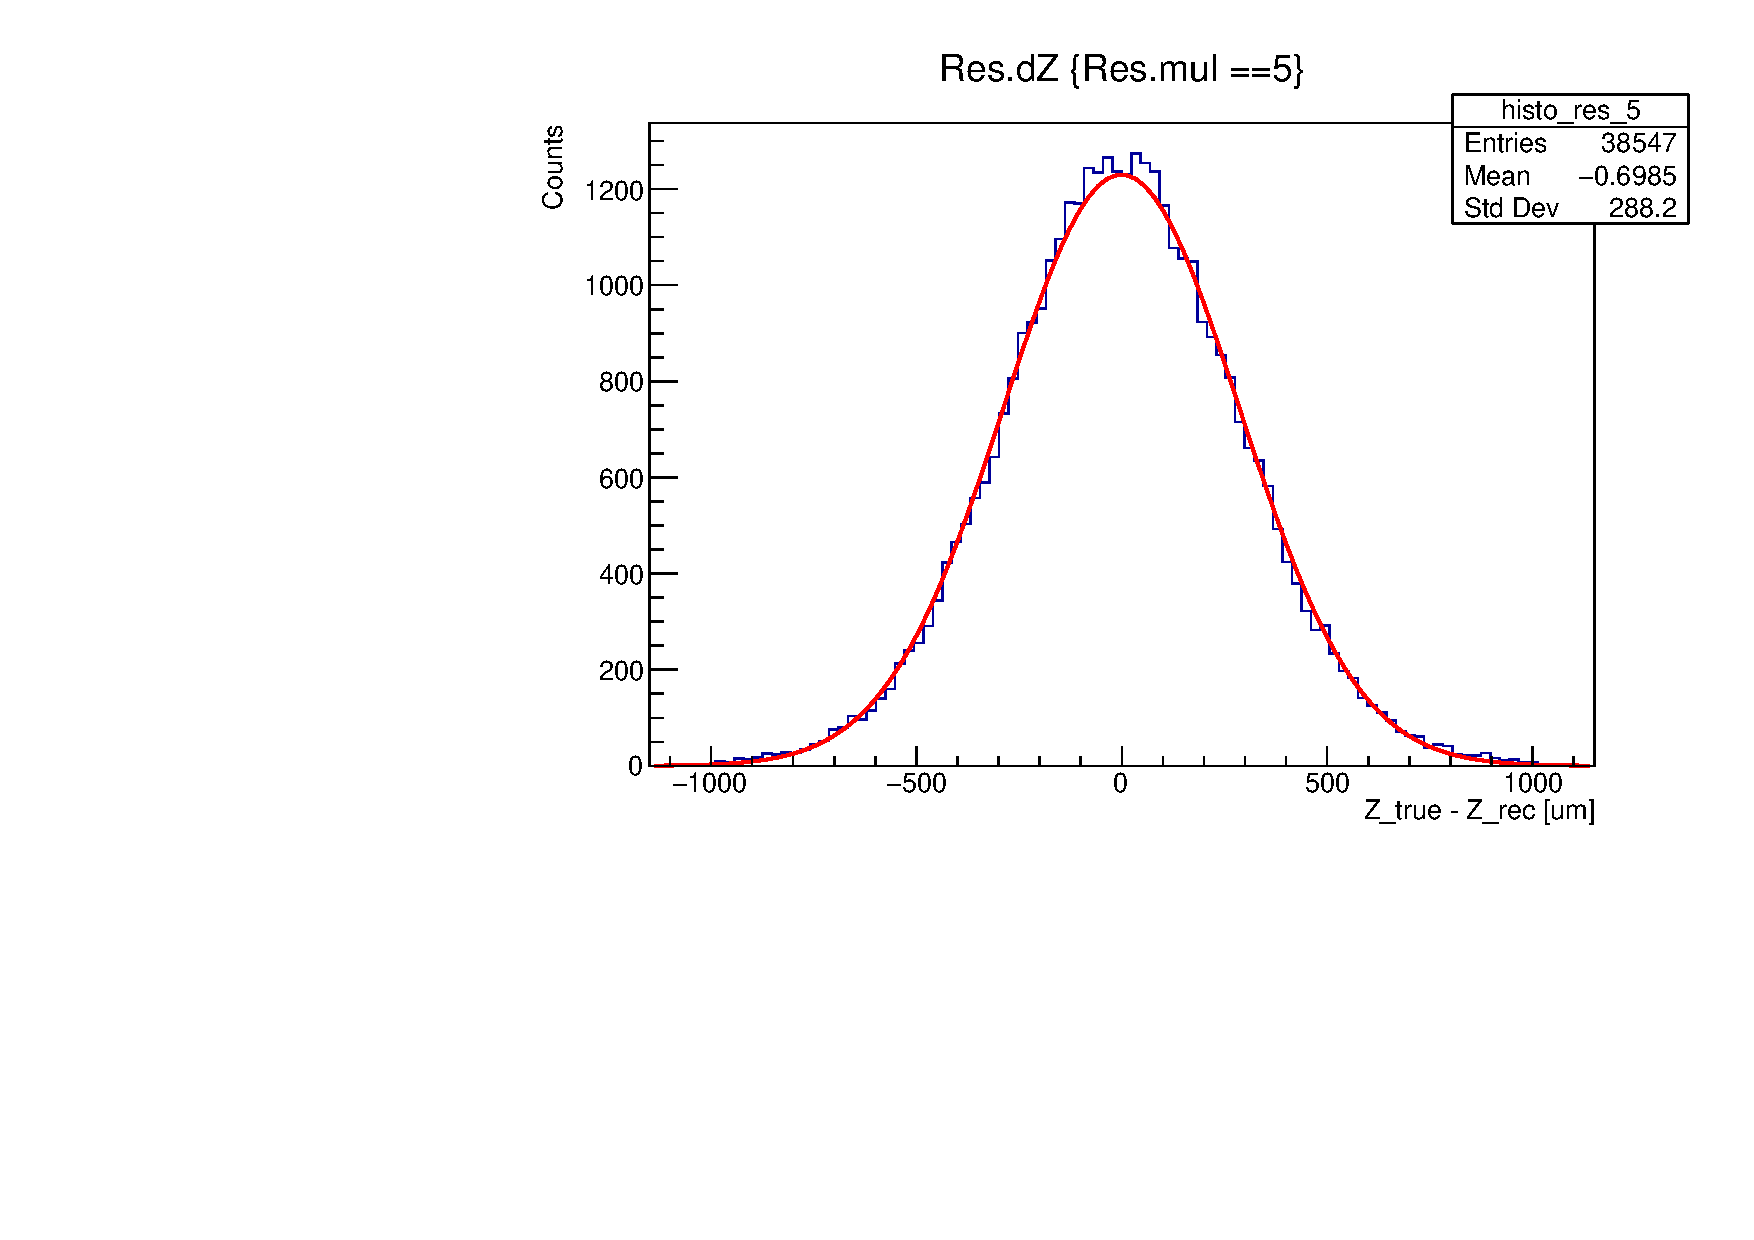
\includegraphics[width=0.4\textwidth]{images/5.pdf}} 
    \subfigure[]{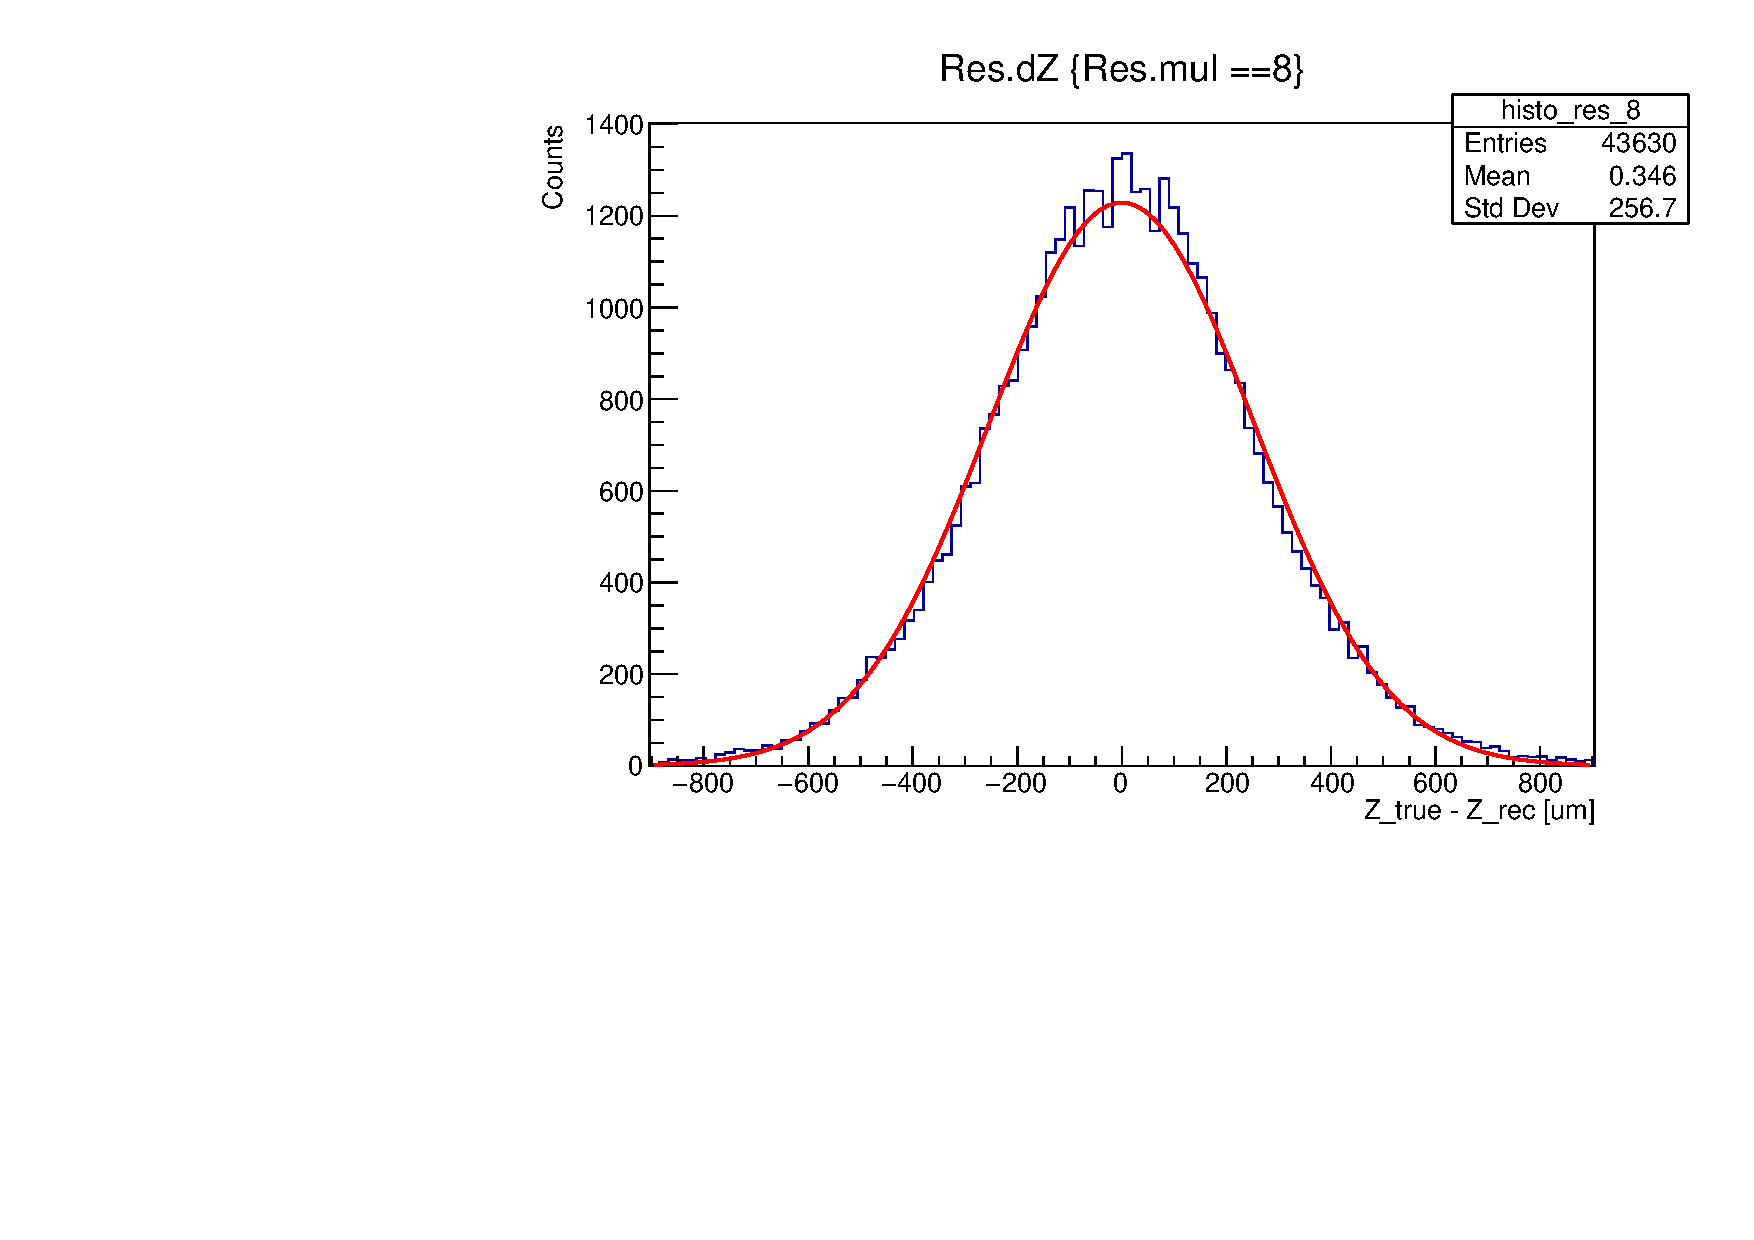
\includegraphics[width=0.4\textwidth]{images/8.pdf}} 
    \subfigure[]{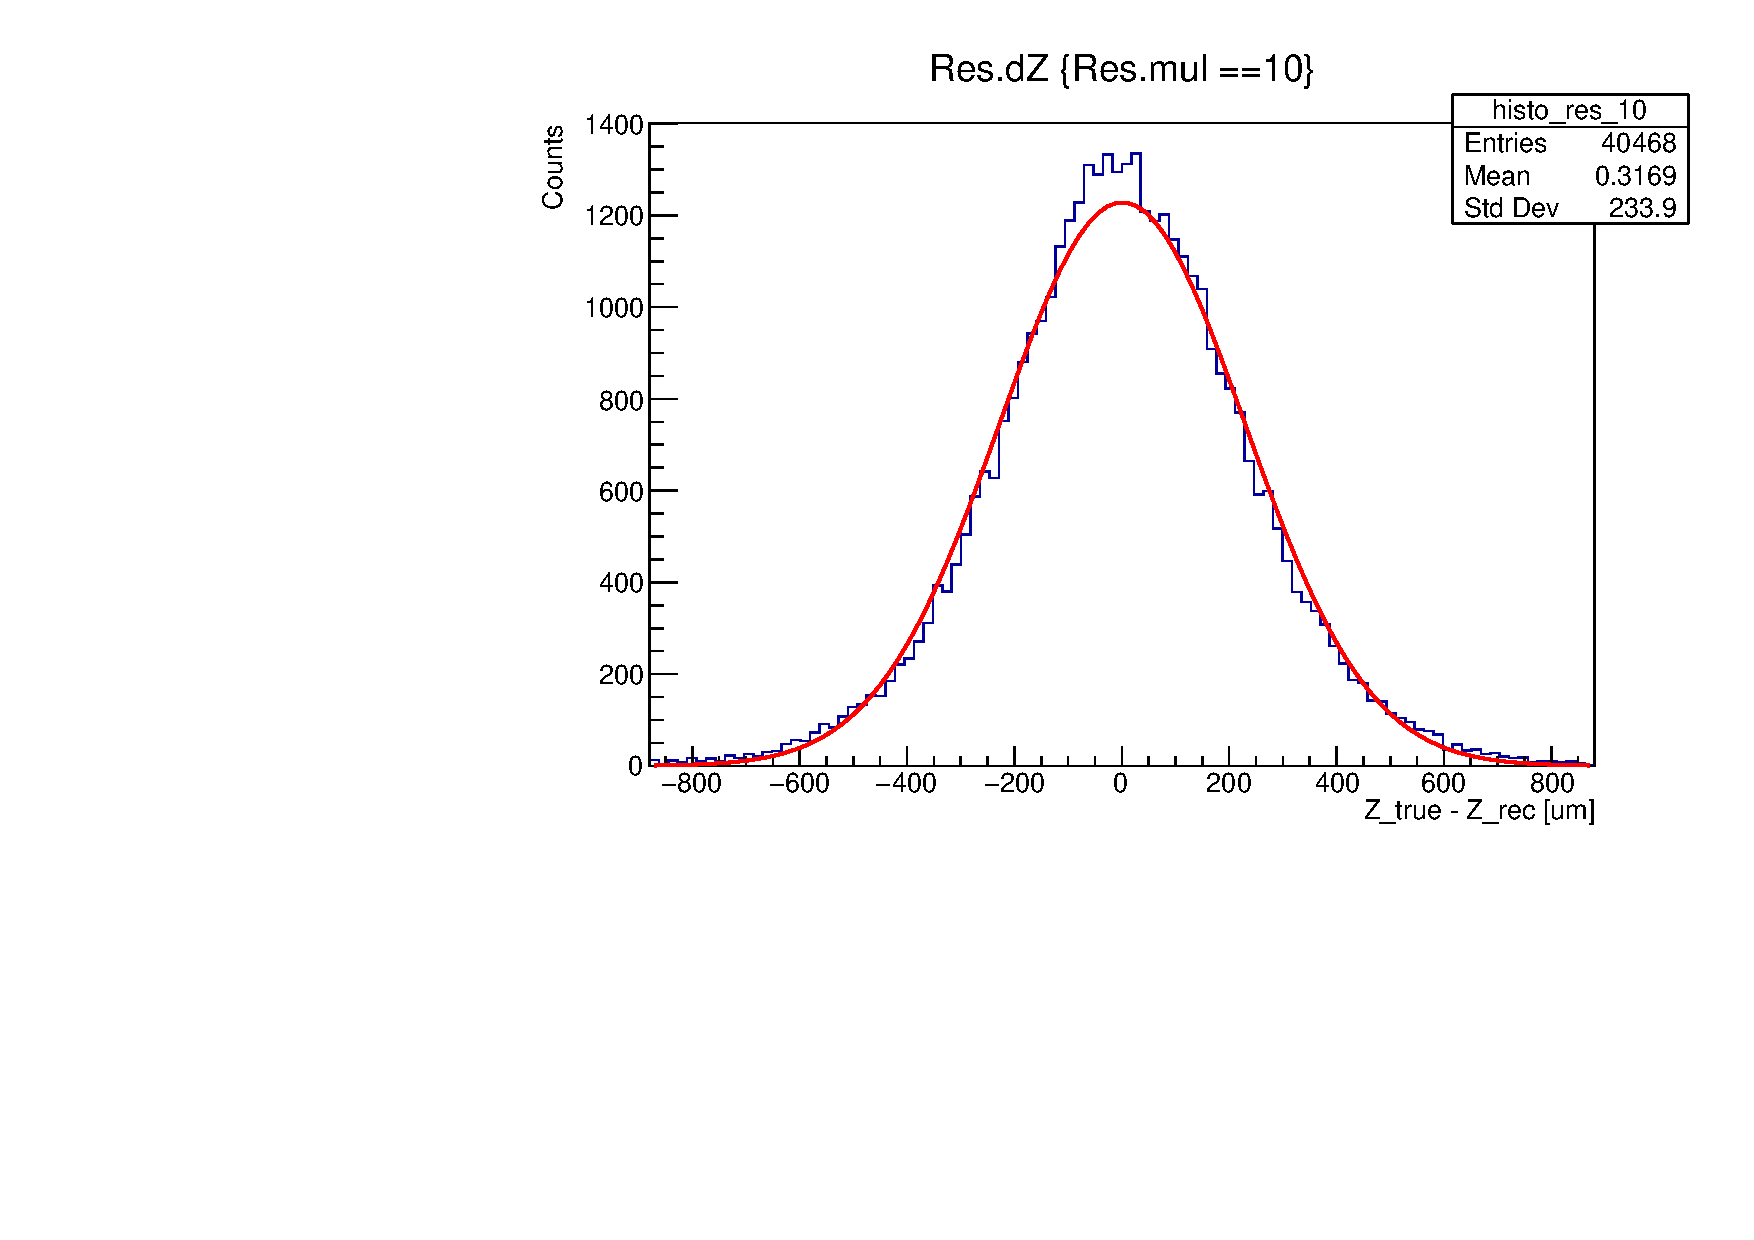
\includegraphics[width=0.4\textwidth]{images/10.pdf}} 
    \subfigure[]{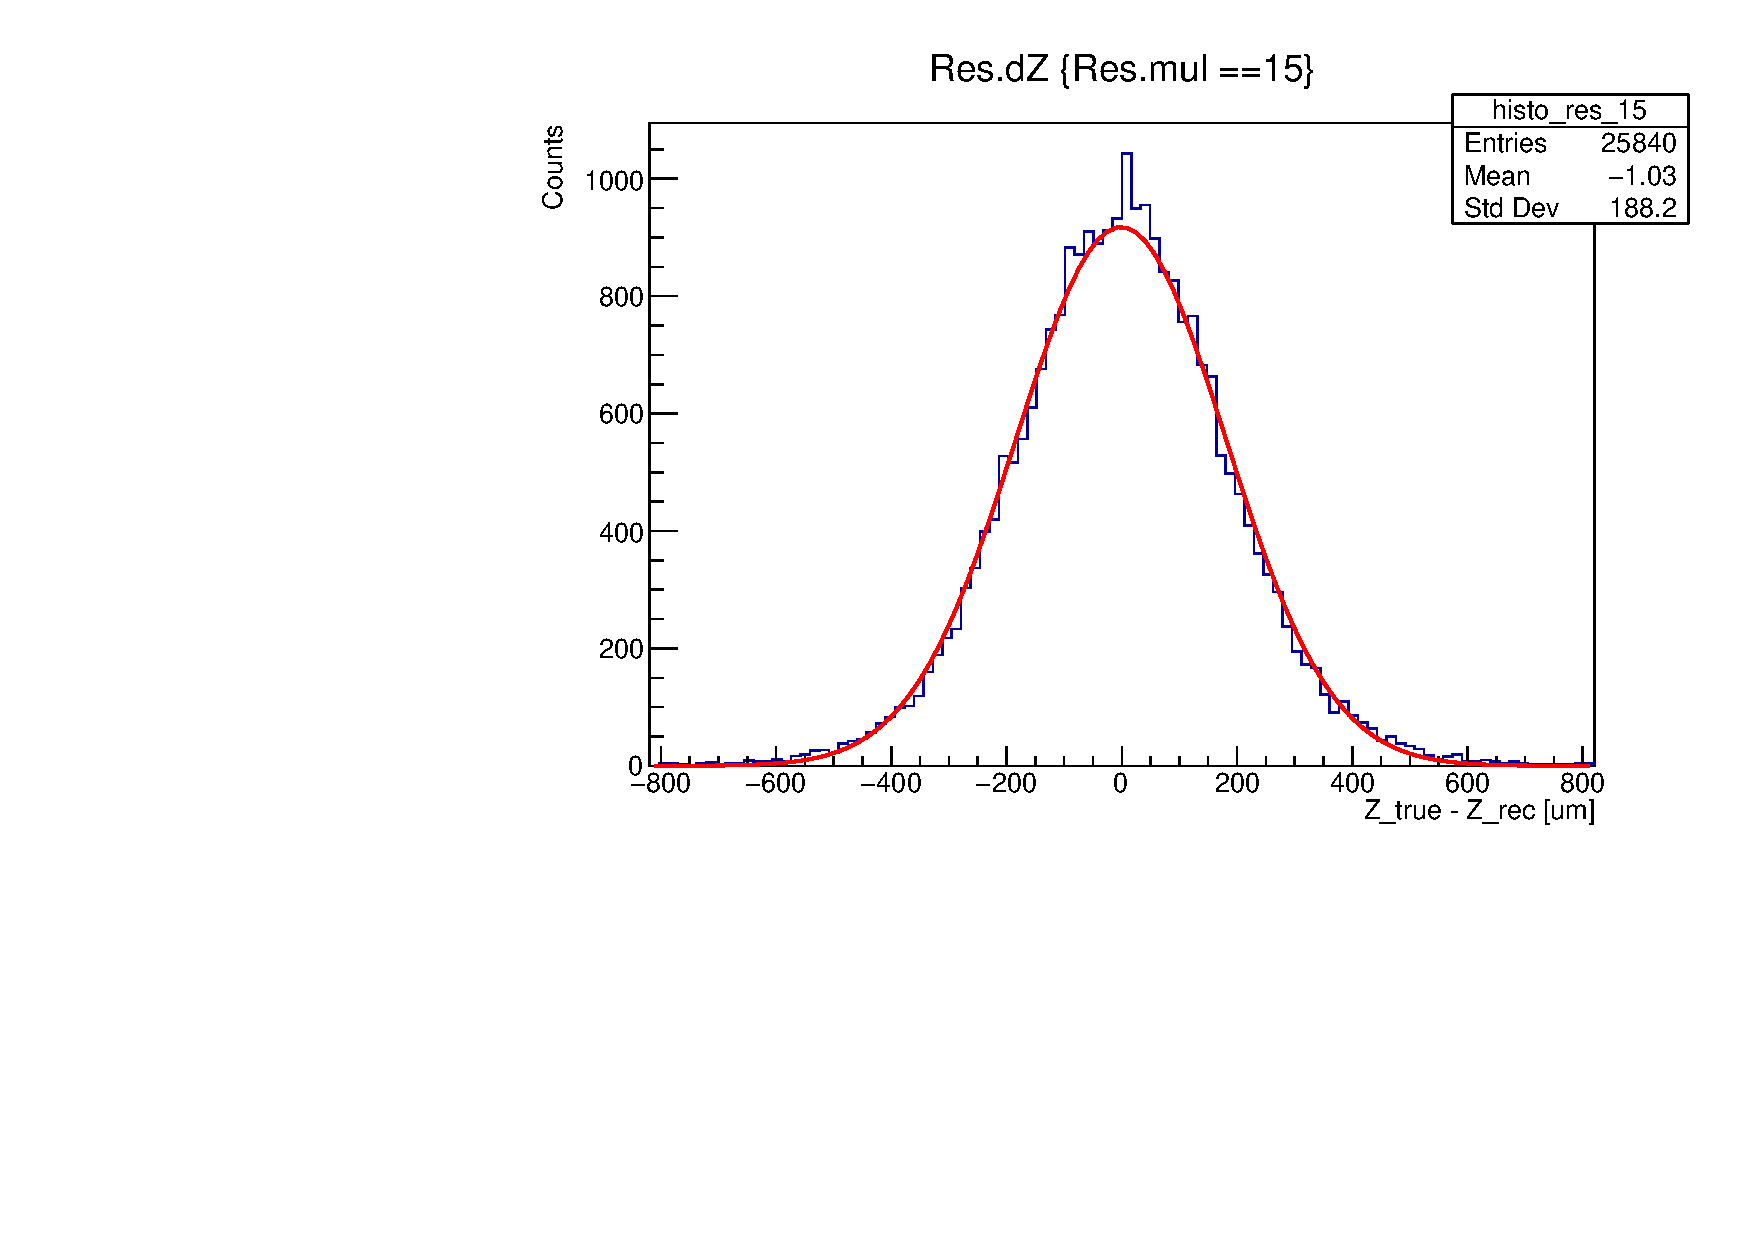
\includegraphics[width=0.4\textwidth]{images/15.pdf}} 
    \subfigure[]{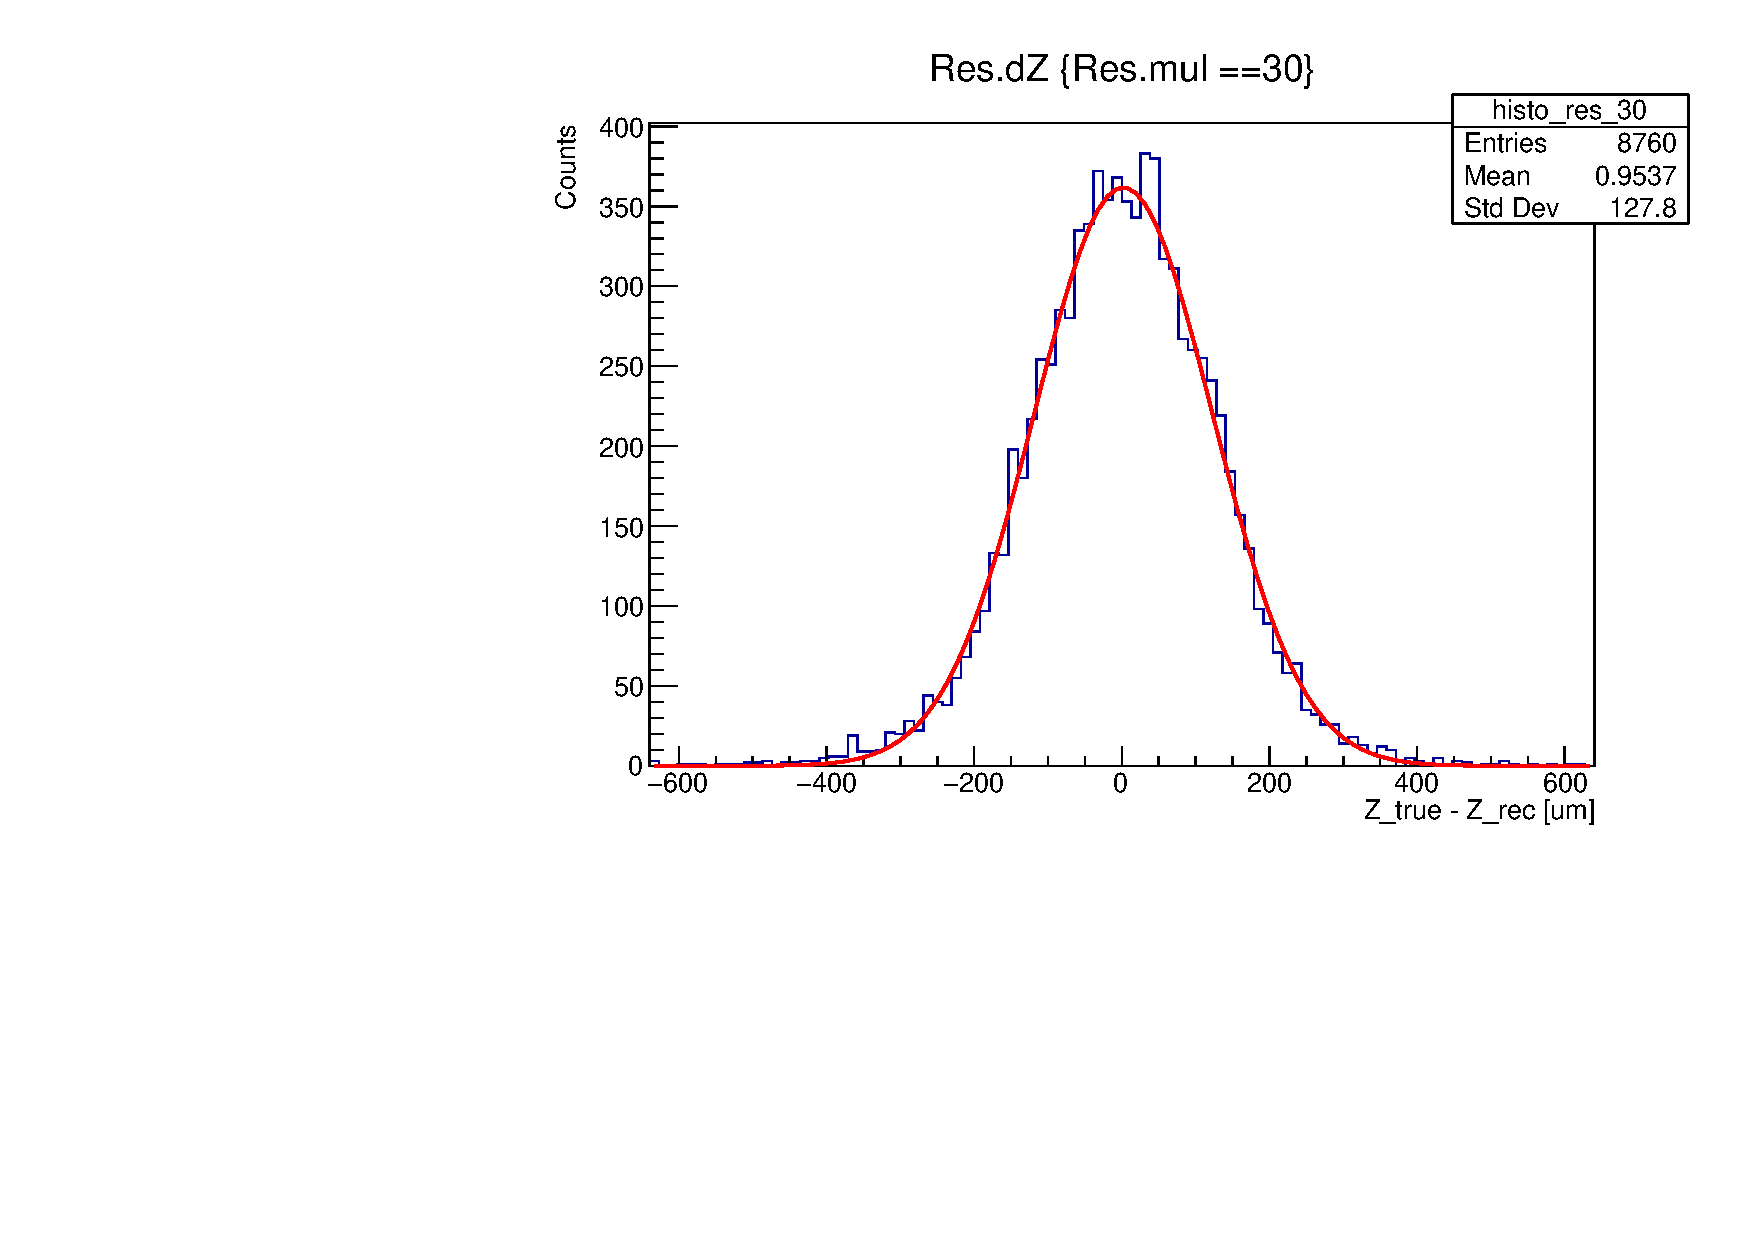
\includegraphics[width=0.4\textwidth]{images/30.pdf}} 
    \subfigure[]{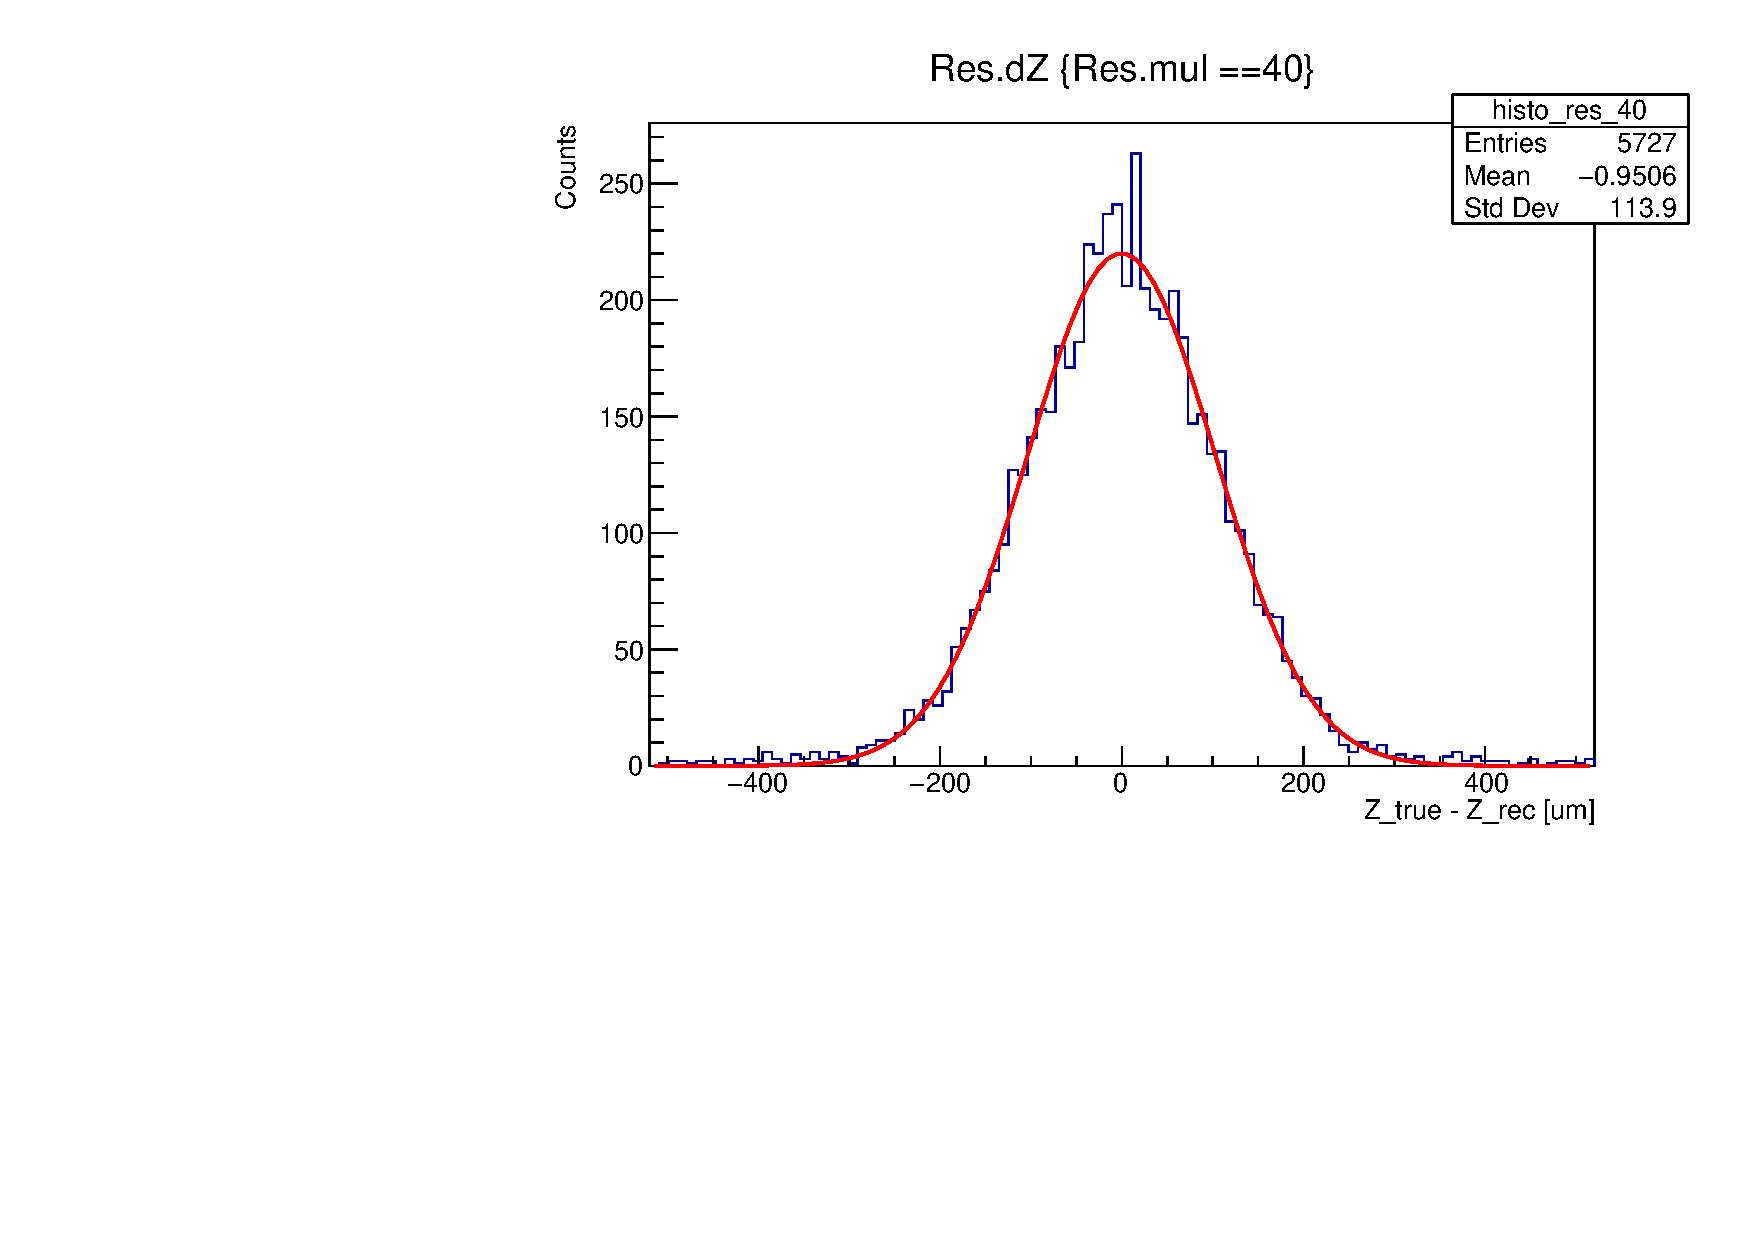
\includegraphics[width=0.4\textwidth]{images/40.pdf}} 
    \subfigure[]{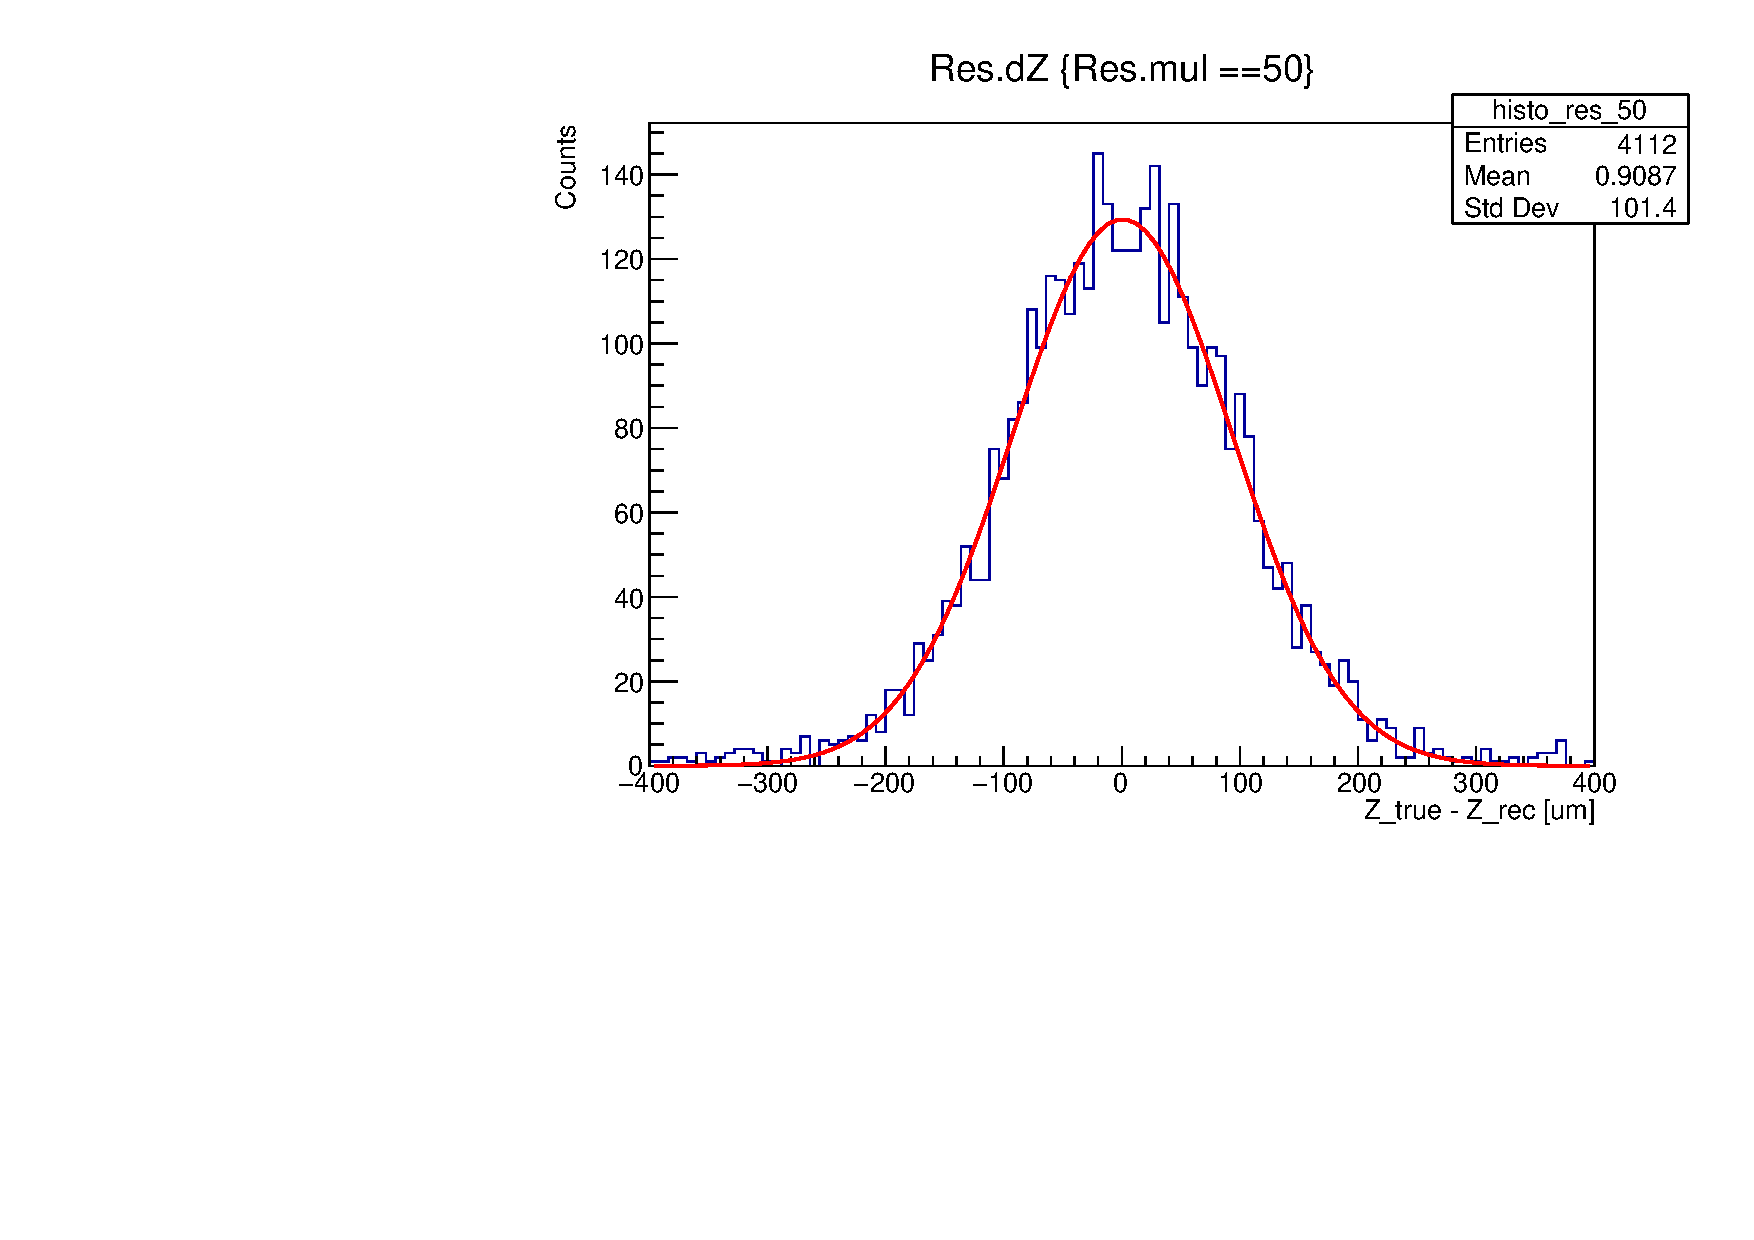
\includegraphics[width=0.4\textwidth]{images/50.pdf}} 
    \label{fig:foobar}
\end{figure}

Si evidenzia come la risoluzione, identificabile nella dispersione di ciascuna gaussiana, diminuisca all'aumentare del valore di molteplicità selezionato. Questo sarà il tema della prossima sottosezione. 

\subsection{Risoluzione vs molteplicità}
Si vuole adesso descrivere l'andamento della risoluzione rispetto al numero di particelle cariche prodotte nella collisione. Come già detto, ci si attende che la prima migliori al crescere della seconda:

\begin{center}
    	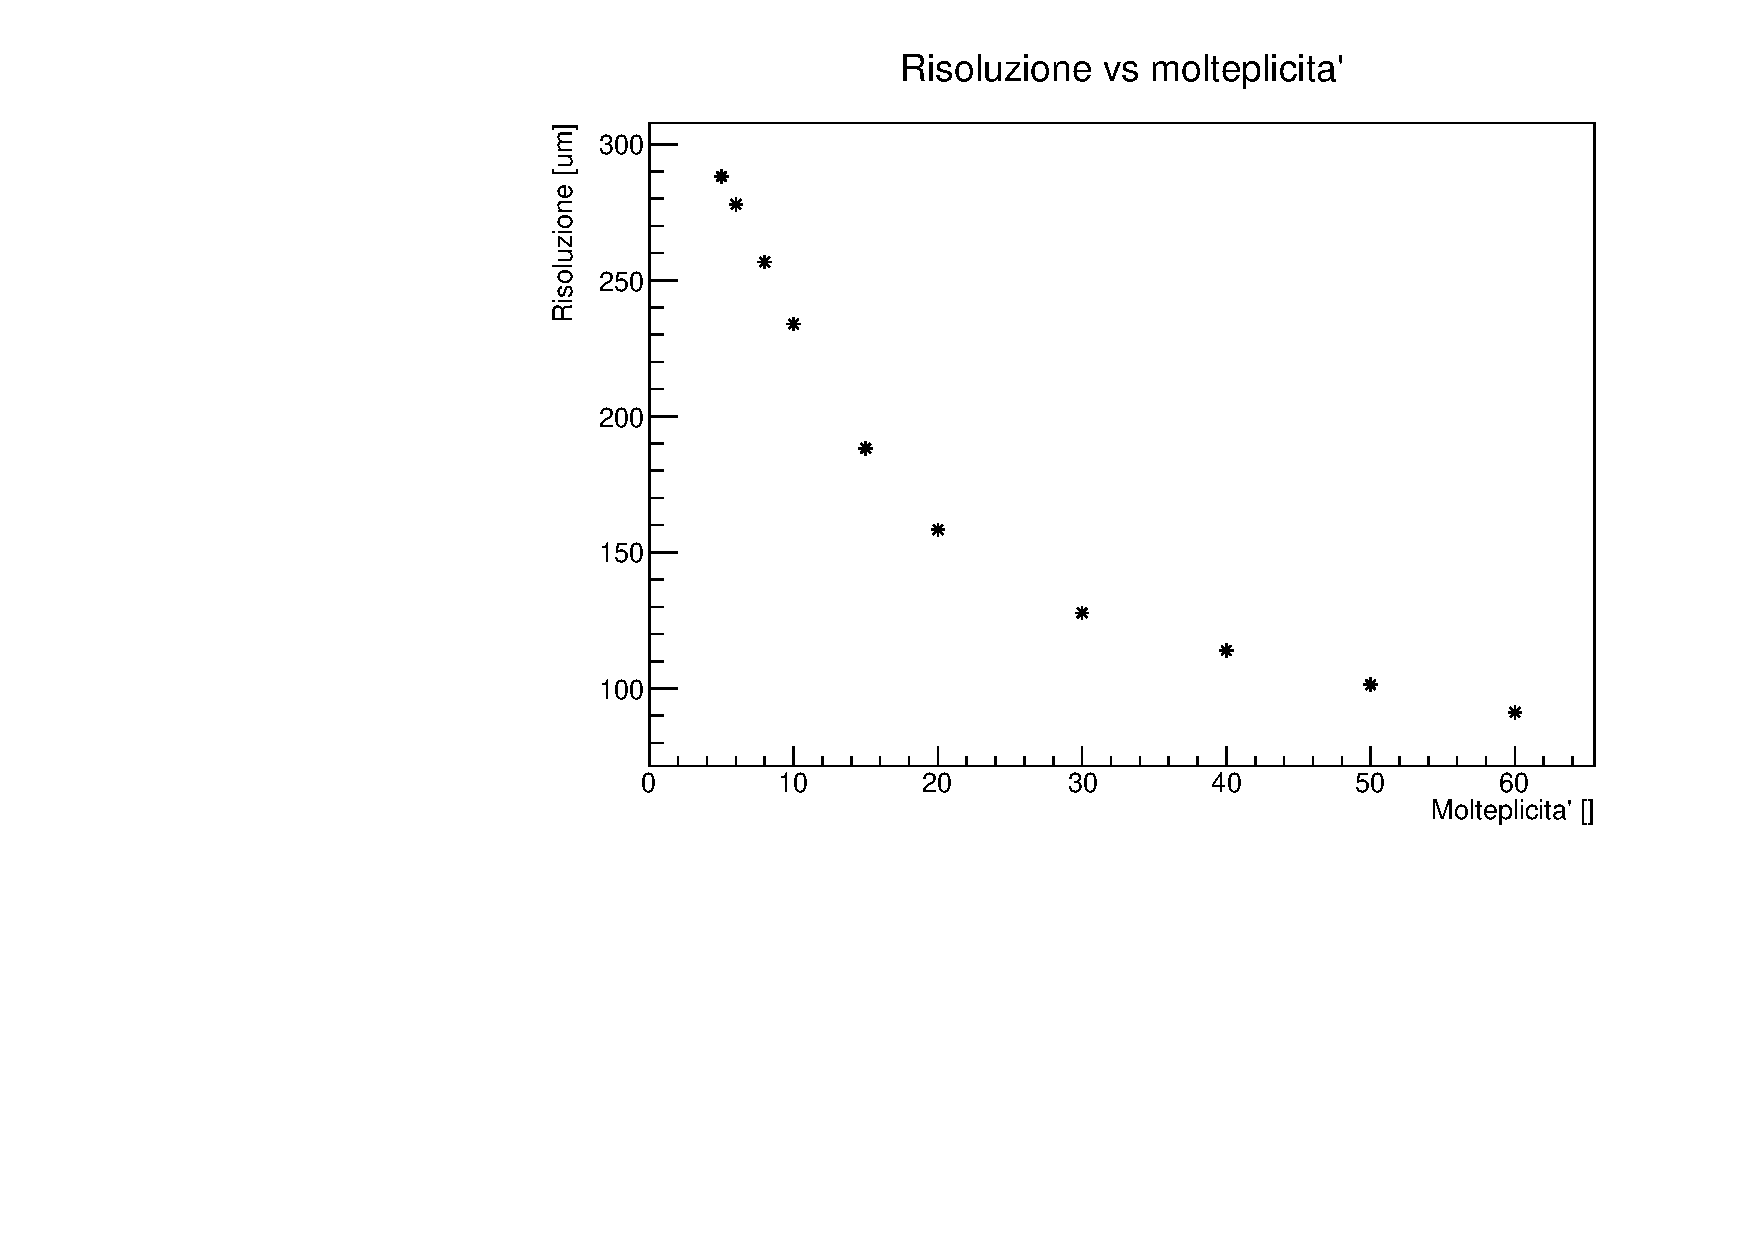
\includegraphics[width=0.55\linewidth]{images/ris_vs_mul.pdf}
\end{center}

Si può concludere che la risoluzione si assesti a valori inferiori a 100 $\mu$m, per valori di molteplicità superiori a 50.

\subsection{Risoluzione vs $Z_{rec}$}
Si vuole adesso descrivere l'andamento della risoluzione rispetto al taglio sulla quota $Z_{true}$ del vertice. Si ottiene il seguente andamento: 

\begin{center}
    	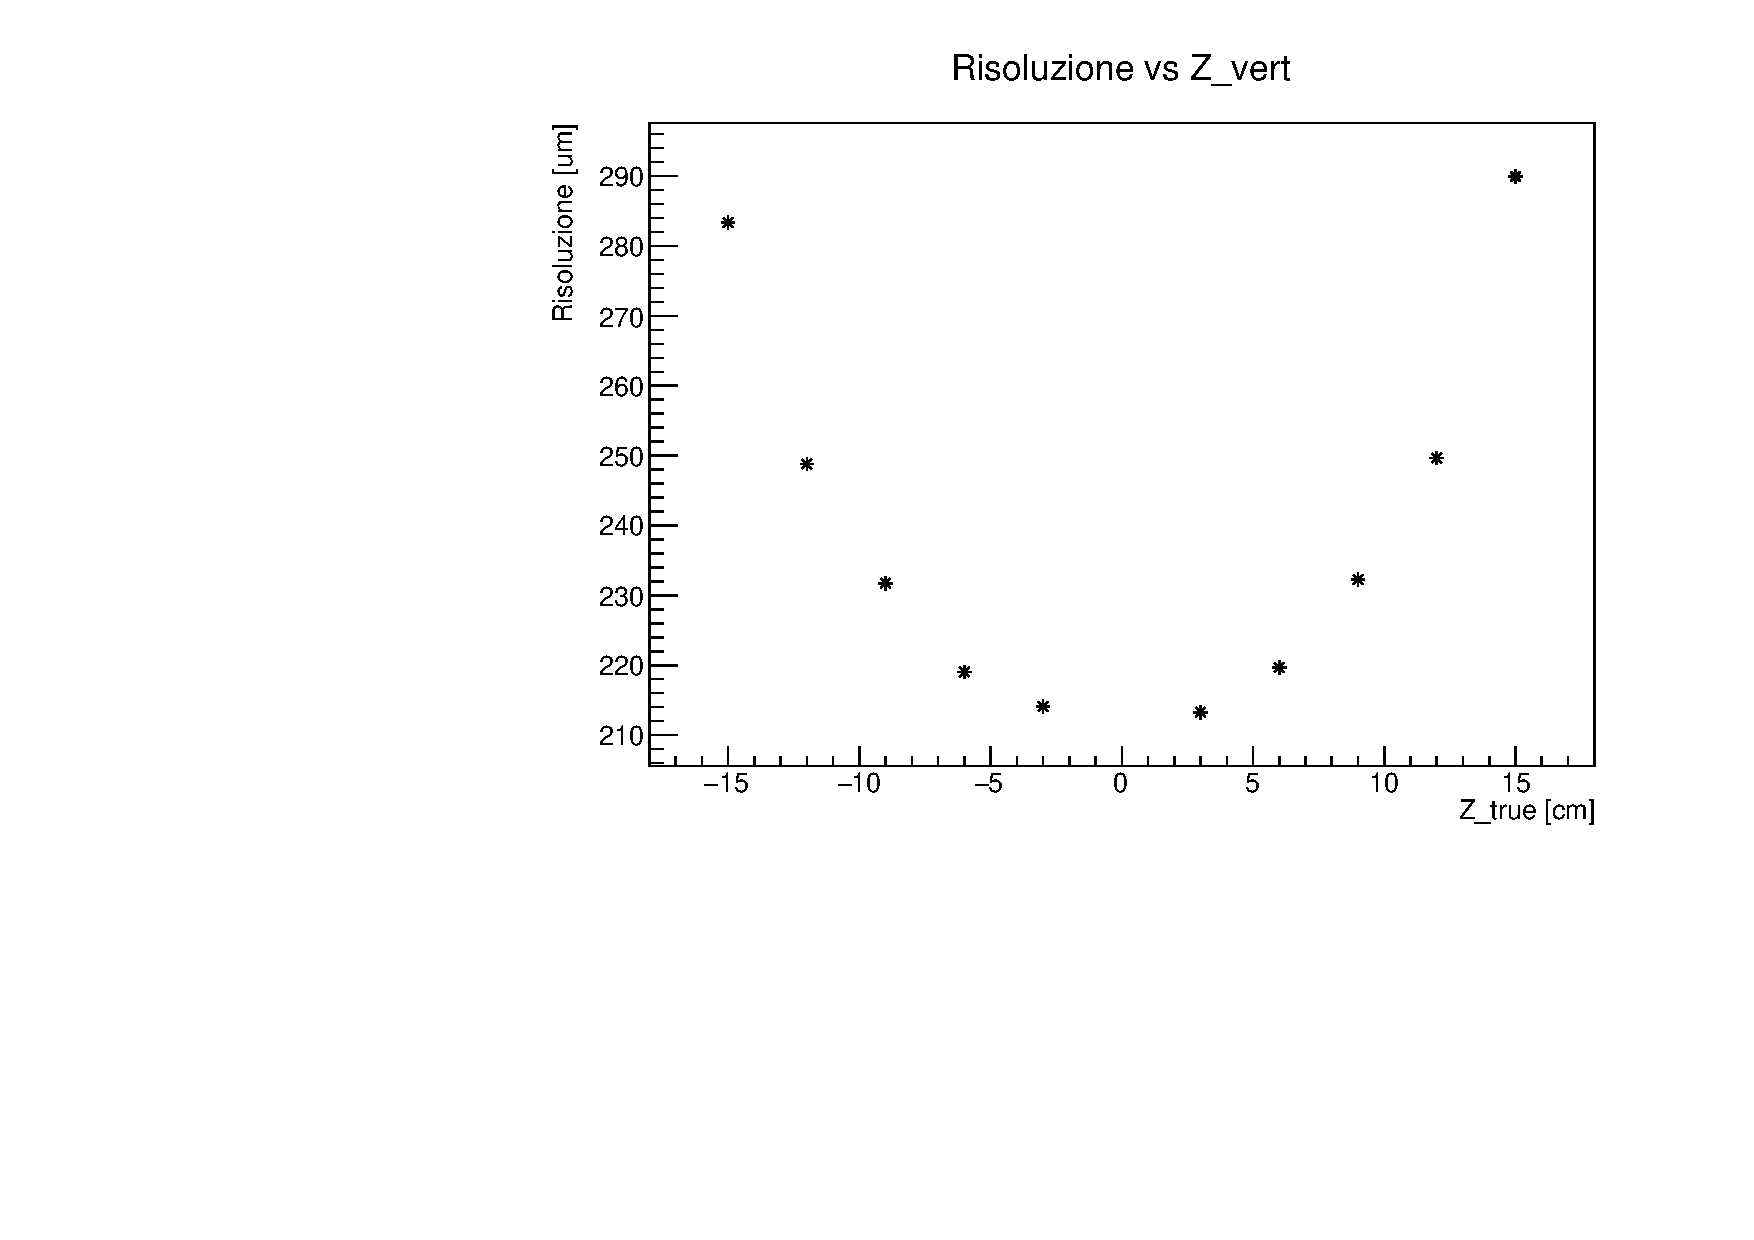
\includegraphics[width=0.55\linewidth]{images/ris_vs_Z.pdf}
\end{center}

Si può osservare come la risoluzione sia migliore per punti centrali al rivelatore e come vada a degradarsi ai bordi.

\subsection{Efficienza vs molteplicità}
Si può definire l'efficienza $\epsilon$ come:
\begin{center}
$\epsilon = \frac {number \ of \ Z_{rec}} {number \ of \ Z_{true}}$
\end{center}
Di seguito si riporta l'andamento di $\epsilon$, al variare della molteplicità:

\begin{center}
    	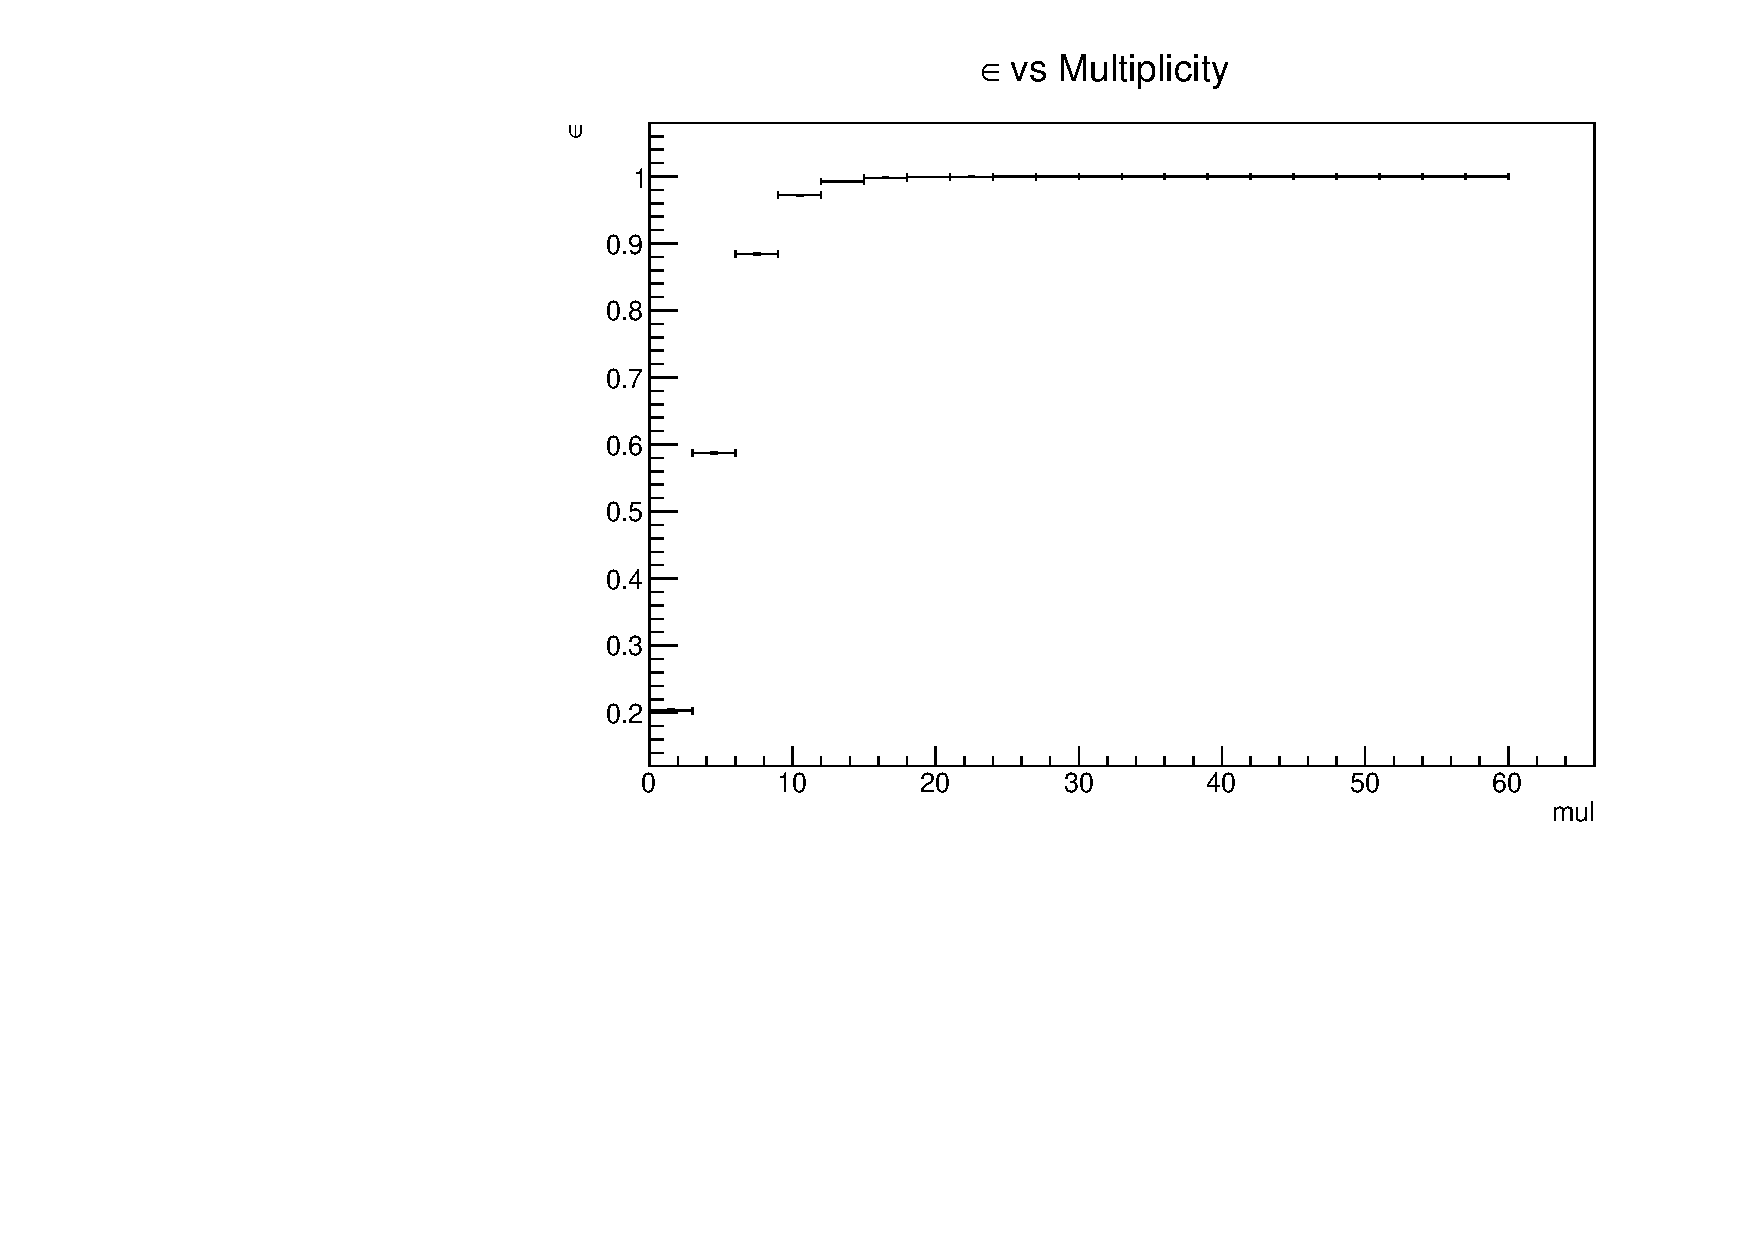
\includegraphics[width=0.55\linewidth]{images/eff_vs_mul.pdf}
\end{center}

Si evidenzia come l'efficienza migliori al crescere della molteplicità.

\subsection{Efficienza vs $Z_{true}$}
Si conclude mostrando l'andamento di $\epsilon$, al variare di $Z_{true}$:

\begin{center}
    	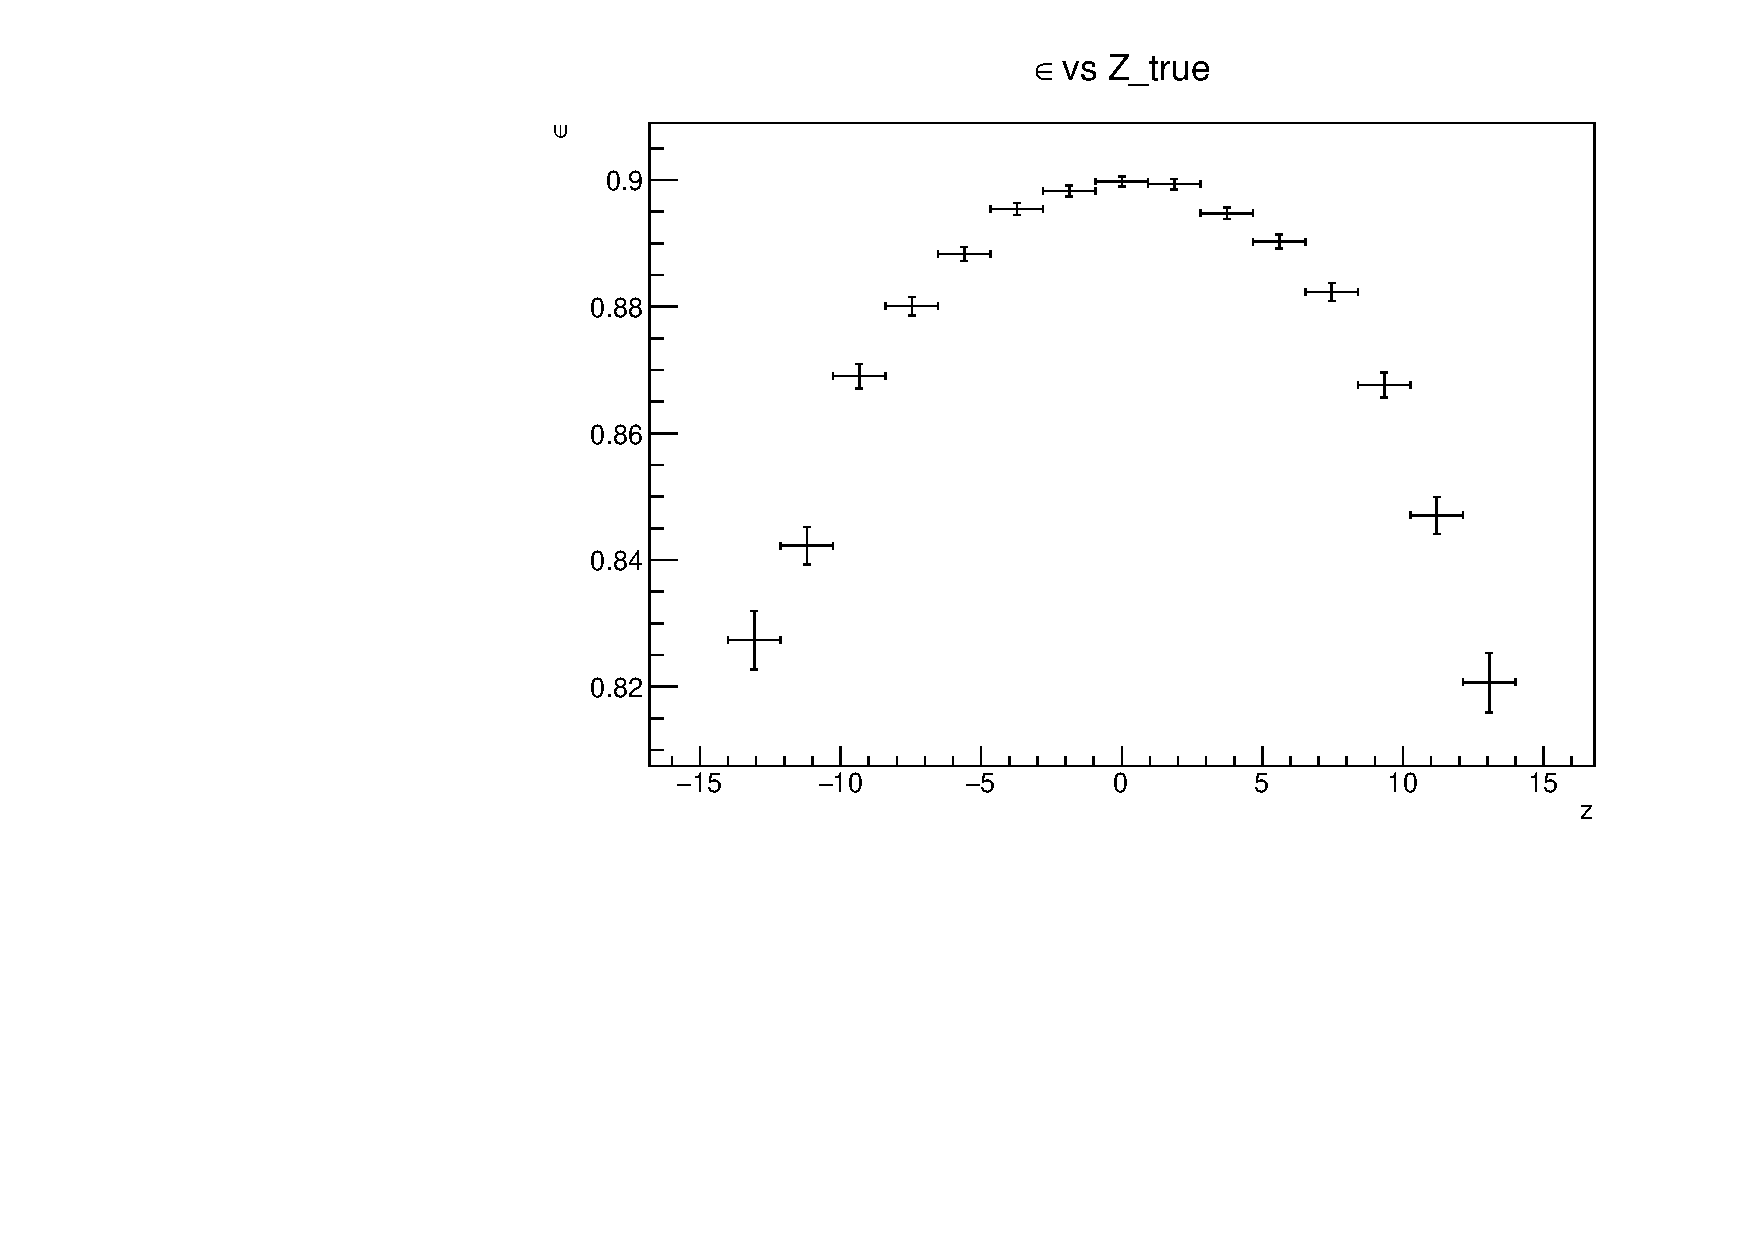
\includegraphics[width=0.55\linewidth]{images/eff_vs_Z.pdf}
\end{center}

Si può notare come, nel presente caso, l'efficienza massima è $\simeq 90\%$ per regioni centrali del rivelatore.
\end{document}